%!TEX encoding = UTF-8 Unicode

\documentclass[a4paper,11pt,obeyspaces,openany]{book}
\usepackage{verbatim}
% L'option 'openany' permet de démarrer un chapitre sur une page paire

% L'option 'obeyspaces' indique au paquetage hyperref de respecter les espaces dans les chemins \path ou \url.
%
% Par exemple : \path{ab cd} est écrit ab cd
% Sans cette option, \path{ab cd} est écrit abcd
% Voir : http://compgroups.net/comp.text.tex/space-in-path-hyperref-package

%-----------------------------------------------------------------------------------------------------------------------*
%                                                                                                                       *
%   « N O I R    E T    B L A N C »    O U    « C O U L E U R »                                                         *
%                                                                                                                       *
%-----------------------------------------------------------------------------------------------------------------------*

%--- Par défaut, l'impression se fait en couleur
\providecommand{\sortieEnCouleur}{true}

%-----------------------------------------------------------------------------------------------------------------------*
%                                                                                                                       *
%   A F F I C H E R    L E    D E T A I L    D E S    S C H É M A S    É L E C T R O N I Q U E S                        *
%                                                                                                                       *
%-----------------------------------------------------------------------------------------------------------------------*

%--- Par défaut, le détail des schémas est affiché
\providecommand\afficherDetailSchema{true}

%-----------------------------------------------------------------------------------------------------------------------*
%                                                                                                                       *
%   E N C O D A G E    D E S    S O U R C E S     :     U T F 8                                                         *
%                                                                                                                       *
%-----------------------------------------------------------------------------------------------------------------------*

%--- Paquetage pour le codage des sources en UTF-8
\usepackage[utf8]{inputenc}

%--- Latex demande ce paquetage pour mieux afficher le caractère "°" et \textquotesingle "'"
\usepackage{textcomp}

%--- Ce paquetage permet d'effectuer certaines césures, et ainsi d'éviter les messages "Overfull \hbox"
\usepackage[T1]{fontenc}

%-----------------------------------------------------------------------------------------------------------------------*
%                                                                                                                       *
%   C H O I X    D E    L A    P O L I C E                                                                              *
%                                                                                                                       *
%-----------------------------------------------------------------------------------------------------------------------*

%\usepackage{lmodern} % for French
%\usepackage{fouriernc}
%\usepackage[scaled=0.875]{helvet}

\usepackage[scaled=0.9,default]{sourcecodepro}
\usepackage[default]{sourcesanspro}

%-----------------------------------------------------------------------------------------------------------------------*
%                                                                                                                       *
%   R É G L A G E S    « F R A N Ç A I S »                                                                              *
%                                                                                                                       *
%-----------------------------------------------------------------------------------------------------------------------*

%--- Paquetage pour imposer les réglages français
%\usepackage[francais]{babel}
\usepackage[frenchb]{babel}

%--- Contrôle de l'indentation et de la séparation des paragraphes
\setlength{\parindent}{0pt} 
%\setlength{\parskip}{1.2ex} % Reporté avant les chapitres

%--- Ajouter une séparation à la fin des itemize
\let\EndItemize\enditemize
\def\enditemize{\EndItemize\vspace{1.2ex}}

%-----------------------------------------------------------------------------------------------------------------------*
%                                                                                                                       *
%   M I S E    E N    P A G E S    D E M A N D É E     P A R     E L L I P S E S                                        *
%                                                                                                                       *
%-----------------------------------------------------------------------------------------------------------------------*

%--- Interligne 1,5 ligne
\usepackage{setspace}
\onehalfspacing

%---------------------------------------------------- Mise en page
% Voir "Une courte introduction à Latex2e", § 6.4

%--- Marge gauche : 2 cm ; le paramètre \hoffset contient cette valeur, moins 1 pouce
%    \hoffset = 2 cm - 2,54 cm = -0,54 cm
\setlength{\hoffset}{-0.54 cm}
%
%%--- Hauteur de la page : 29,7 cm
%\setlength{\paperheight}{29.7 cm}
%
%--- Largeur de la page
%\setlength{\paperwidth}{18 cm}
%
%%--- Marges supplémentaires, différenciées pour les pages gauches et droites ; ici, aucune.
%\setlength{\oddsidemargin }{0 cm}
%\setlength{\evensidemargin}{0 cm}
%
%--- Largeur du texte
\setlength{\textwidth}{14cm}
%
%%--- Marge haute : 2,8 cm ; le paramètre \voffset contient cette valeur, moins 1 pouce
%%    \voffset = 2,8 cm - 2,54 cm = 0,26 cm
%\setlength{\voffset}{0.26 cm}
%
%%--- Distance entre la marge haute et l'en-tête : 0 cm
%\setlength{\topmargin}{0 cm}
%
%%--- Hauteur de l'en-tête de chaque page : 1 cm
%\setlength{\headheight}{1 cm}
%
%%--- Distance entre l'en-tête de chaque page et le corps : 0,5 cm
%\setlength{\headsep}{0.5 cm}
%
%%--- Hauteur du corps
%%    \textheight = 29,7 cm - 2,8 cm - 2,8 cm - 1,5 cm = 22,6 cm
%\setlength{\textheight}{22.6 cm}
%
%%--------------------- Changer la taille des notes en bas de page
%%  footnotesize ---> small
%
%\let\oldfootnotesize\footnotesize
%\renewcommand*{\footnotesize}{\oldfootnotesize\small}

%-----------------------------------------------------------------------------------------------------------------------*
%                                                                                                                       *
%   T R A C E R    U N E    L I G N E    H O R I Z O N T A L E                                                          *
%                                                                                                                       *
%-----------------------------------------------------------------------------------------------------------------------*

\newcommand\ligne{\noindent\makebox[\linewidth]{\rule{\textwidth}{0.5pt}}}

%-----------------------------------------------------------------------------------------------------------------------*
%                                                                                                                       *
%   P A Q U E T A G E    « I F T H E N »                                                                                *
%                                                                                                                       *
%-----------------------------------------------------------------------------------------------------------------------*

%--- Ce paquetage permet d'effectuer des tests : \ifthenelse{test}{bloc then}{bloc else}
\usepackage{ifthen}

%-----------------------------------------------------------------------------------------------------------------------*
%                                                                                                                       *
%   G E S T I O N    D E    L ' I N D E X                                                                               *
%                                                                                                                       *
%-----------------------------------------------------------------------------------------------------------------------*

% http://www.cuk.ch/articles/4097
% http://www.tuteurs.ens.fr/logiciels/latex/makeindex.html
% http://linux.die.net/man/1/makeindex
%
% Attention ! Les deux commandes suivantes, ainsi que le \printindex placé plus bas ne
% sont pas suffisants pour construire l'index : il faut utiliser l'utilitaire "makeIndex"
% Voir le fichier de commande "build.command"
\usepackage{makeidx}
\makeindex

%-----------------------------------------------------------------------------------------------------------------------*
%                                                                                                                       *
%   H Y P E R R E F                                                                                                     *
%                                                                                                                       *
%-----------------------------------------------------------------------------------------------------------------------*


%--- Pour les hyperliens, et le contrôle de la génération PDF 
\usepackage[pagebackref]{hyperref}

\hypersetup{pdftitle      = {PLM}}
\hypersetup{pdfauthor     = {Pierre Molinaro}}

\hypersetup{colorlinks    = true}
\hypersetup{anchorcolor   = black}
\hypersetup{filecolor     = black}
\hypersetup{menucolor     = black}
\hypersetup{plainpages    = false}
\hypersetup{pdfstartview  = FitH}
\hypersetup{pdfpagelayout = OneColumn}

%--- Contrôle des références de la bibliographie ; avec ces lignes, les pages où chaque item de la biblio
%    est appelée sont insérées à la fin de chaque entrée.
%\hypersetup{backref        = page}

\renewcommand*{\backrefalt}[4]{
  \ifcase #1 % case: not cited
    \ifthenelse{\equal{\sortieEnCouleur}{true}}{\textcolor{red}{\textbf{(non cité)}}}{\textbf{(non cité)}}. 
  \or % case: cited on exactly one page 
    (cité page #2).% 
  \else % case: cited on multiple pages 
    (cité pages #2). 
  \fi
} 
\renewcommand*{\backreftwosep}{ et }
\renewcommand*{\backreflastsep}{ et }


%--- Les hyperliens sont colorés en bleu dans la phase de mise au point, ils sont ainsi mieux visibles
\ifthenelse{\equal{\sortieEnCouleur}{true}}{
  \hypersetup{linkcolor  = blue}
  \hypersetup{urlcolor   = blue}
  \hypersetup{citecolor  = blue}
}{
  \hypersetup{linkcolor  = black}
  \hypersetup{urlcolor   = black}
  \hypersetup{citecolor  = black}
}

%---------------------------------------------------- Numéro de section
% Par défaut, une section est affichée avec son numéro de chapitre : par exemple : 2.1 Titre
% Les Éditions Ellipses précisent que le numéro de chapitre ne doit pas apparaître, ni dans le corps, ni dans l'en-tête
% Voir http://help-csli.stanford.edu/tex/latex-sections.shtml
% La solution suivante affecte aussi les sous-sections, ainsi que la table des matières.
%\renewcommand\thesection {\arabic{section}}

%---------------------------------------------------- Affichage des numéros de section
% C'est à dire les numéros qui sont affichées pour \section, \subsection, ...
% Par défaut, l'affichage se fait jusqu'au niveau 2 (\subsection)
% Avec cette commande, on va jusqu'au niveau \subsubsection.
%\setcounter{secnumdepth}{3}

%---------------------------------------------------- Définition de subsubsubsection
% http://forum.mathematex.net/latex-f6/definir-un-subsubsubsection-t4031.html
\makeatletter
\newcounter{subsubsubsection}[subsubsection]
\renewcommand\thesubsubsubsection{\thesubsubsection .\@alph\c@subsubsubsection}
\newcommand\subsubsubsection{\@startsection{subsubsubsection}{4}{\z@}%
                                     {-3.25ex\@plus -1ex \@minus -.2ex}%
                                     {1.5ex \@plus .2ex}%
                                     {\normalfont\normalsize\bfseries}}
\newcommand*\l@subsubsubsection{\@dottedtocline{3}{10.0em}{4.1em}}
\newcommand*{\subsubsubsectionmark}[1]{}
\makeatother

\makeatletter
\def\toclevel@subsubsubsection{4}
\makeatother

%------------------------------------------------------------------------------------------ RÉFÉRENCES À UN TABLEAU
% La référence au tableau "nom-du-tableau" est définie par \labelTableau{nom-du-tableau}
\newcommand\labelTableau[1]{\label{tab:#1}}
% Latex autorise deux types d'appel à une référence \ref{tab:nom-du-tableau} et \pageref{tab:nom-du-tableau}

% \refTableau{}{nom-du-tableau} ---> "tableau x.y"   où x.y est le n° du tableau
\newcommand\refTableau[1]{\hyperref[tab:#1]{tableau \ref*{tab:#1}}}

% \refTableauSansPrefixe{}{nom-du-tableau} ---> "x.y"   où x.y est le n° du tableau
\newcommand\refTableauSansPrefixe[1]{\hyperref[tab:#1]{\ref*{tab:#1}}}

% \refTableauPage{}{nom-du-tableau} ---> "tableau x.y page n"   où x.y est le n° du tableau
\newcommand\refTableauPage[1]{\hyperref[tab:#1]{tableau \ref*{tab:#1} page \pageref{tab:#1}}}

% \refTableauPageSansPrefixe{}{nom-du-tableau} ---> "x.y page n"   où x.y est le n° du tableau
\newcommand\refTableauPageSansPrefixe[1]{\hyperref[tab:#1]{\ref*{tab:#1} page \pageref{tab:#1}}}

%------------------------------------------------------------------------------------------ RÉFÉRENCES À UNE FIGURE
% La référence au tableau "nom-de-la-figure" est définie par \labelFigure{nom-de-la-figure}
\newcommand\labelFigure[1]{\label{fig:#1}}
% Latex autorise deux types d'appel à une référence \ref{fig:nom-de-la-figure} et \pageref{fig:nom-de-la-figure}

% \refFigure{}{nom-de-la-figure}   ---> "figure x.y"   où x.y est le n° de la figure
% \refFigure{z}{nom-de-la-figure}  ---> "figure x.y.z" où x.y est le n° de la figure
\newcommand\refFigure[2]{\hyperref[fig:#2]{figure \ref*{fig:#2}{\ifthenelse{\equal{#1}{}}{}{.#1}}}}

% \refFigureSansPrefixe{}{nom-de-la-figure}   ---> "x.y"   où x.y est le n° de la figure
% \refFigureSansPrefixe{z}{nom-de-la-figure}  ---> "x.y.z" où x.y est le n° de la figure
\newcommand\refFigureSansPrefixe[2]{\hyperref[fig:#2]{\ref*{fig:#2}{\ifthenelse{\equal{#1}{}}{}{.#1}}}}

% \refFigurePage{}{nom-de-la-figure}   ---> "figure x.y page n"   où x.y est le n° de la figure
% \refFigurePage{z}{nom-de-la-figure}  ---> "figure x.y.z page n" où x.y est le n° de la figure
\newcommand\refFigurePage[2]{\hyperref[fig:#2]{figure \ref*{fig:#2}{\ifthenelse{\equal{#1}{}}{}{.#1}} page \pageref{fig:#2}}}

% \refFigurePageSansPrefixe{}{nom-de-la-figure}   ---> "x.y page n"   où x.y est le n° de la figure
% \refFigurePageSansPrefixe{z}{nom-de-la-figure}  ---> "x.y.z page n" où x.y est le n° de la figure
\newcommand\refFigurePageSansPrefixe[2]{\hyperref[fig:#2]{\ref*{fig:#2}{\ifthenelse{\equal{#1}{}}{}{.#1}} page \pageref{fig:#2}}}

%------------------------------------------------------------------------------------------ RÉFÉRENCES À UN EXERCICE
% Les exercices sont toujours définis au niveau des sous-sections.
% Au lieu d'écrire \subsection{titre-exercice}, on écrit \subsectionExercice{titre-exercice}{label-exercice}
% De cette façon, un label est défini pour chaque exercice.
\newcommand\subsectionExercice[2]{\subsection{#1}\label{exo:#2}}

% \refExercicePage{label-exercice} ---> "exercice x.y page n" où x.y est le n° de l'exercice
\newcommand\refExercicePage[1]{\hyperref[exo:#1]{exercice \ref*{exo:#1} page \pageref{exo:#1}}}

%------------------------------------------------------------------------------------------ RÉFÉRENCES À UN CHAPITRE
% Au lieu d'écrire \chapter{titre-chapitre}, on écrit \chapterLabel{titre-chapitre}{label-chapitre}
\newcommand \chapterLabel[2]{\chapter{#1}\label{chapter:#2}}


% \refChapter{label-chapter} ---> "chapitre n"
\newcommand \refChapter[1]{\hyperref[chapter:#1]{chapitre \ref*{chapter:#1}}}

\newcommand \refChapterPage[1]{\hyperref[chapter:#1]{chapitre \ref*{chapter:#1} page \pageref{chapter:#1}}}

%------------------------------------------------------------------------------------------ RÉFÉRENCES À UNE SECTION
% Au lieu d'écrire \section{titre-section}, on écrit \sectionLabel{titre-section}{label-section}
\newcommand \sectionLabel[2]{\section{#1}\label{sec:#2}}


% \refSectionPage{label-section} ---> "section x.y page n"   où x.y est le n° de la section
\newcommand\refSectionPage[1]{\hyperref[sec:#1]{section \ref*{sec:#1} page \pageref{sec:#1}}}

%------------------------------------------------------------------------------------------ RÉFÉRENCES À UNE SUB-SECTION
% Au lieu d'écrire \subsection{titre-section}, on écrit \subsectionLabel{titre-section}{label-section}
\newcommand \subsectionLabel[2]{\subsection{#1}\label{subsec:#2}}


% \refSubsectionPage{label-section} ---> "section x.y page n"   où x.y est le n° de la sub-section
\newcommand\refSubsectionPage[1]{\hyperref[subsec:#1]{section \ref*{subsec:#1} page \pageref{subsec:#1}}}

%------------------------------------------------------------------------------------------ RÉFÉRENCES À UNE SUB-SUB-SECTION
% Au lieu d'écrire \subsubsection{titre-section}, on écrit \subsubsectionLabel{titre-section}{label-section}
\newcommand \subsubsectionLabel[2]{\subsubsection{#1}\label{subsubsec:#2}}


% \refSubsectionPage{label-section} ---> "page n"   où n est la page de la sub-sub-section
\newcommand\refSubsubsectionPage[1]{\hyperref[subsubsec:#1]{section \ref*{subsubsec:#1} page \pageref{subsubsec:#1}}}

%------------------------------------------------------------------------------------------ RÉFÉRENCES À UNE SUB-SUB-SUB-SECTION
% Au lieu d'écrire \subsubsubsection{titre-section}, on écrit \subsubsubsectionLabel{titre-section}{label-section}
\newcommand \subsubsubsectionLabel[2]{\subsubsubsection{#1}\label{subsubsubsec:#2}}


% \refSubsubsubsectionPage{label-section} ---> "page n"   où n est la page de la sub-sub-section
\newcommand\refSubsubsubsectionPage[1]{\hyperref[subsubsubsec:#1]{page \pageref{subsubsubsec:#1}}}

%------------------------------------------------------------------------------------------ RÉFÉRENCES À UNE ÉQUATION
% Pour une équation, au lieu d'écrire \label{label-equation}, on écrit \labelEquation{label-equation}
\newcommand \labelEquation[1]{\label{equ:#1}}

% \refEquationPage{label-equation} ---> "équation x.y page n" où x.y est le n° de l'équation
\newcommand\refEquationPage[1]{\hyperref[equ:#1]{équation \ref*{equ:#1} page \pageref{equ:#1}}}

% \refEquation{label-equation} ---> "équation x.y" où x.y est le n° de l'équation
\newcommand\refEquation[1]{\hyperref[equ:#1]{équation \ref*{equ:#1}}}

%------------------------------------------------------------------------------------------ RÉFÉRENCES À UN SYSTÈME
% Pour latex, équation et systèmes (d'équation) sont numérotés grâce au même compteur ; on distingue les deux
% pour les référencements soient différents
% Pour un système, au lieu d'écrire \label{label-systeme}, on écrit \labelSystème{label-systeme}
\newcommand \labelSysteme[1]{\label{syst:#1}}

% \refSysteme{label-systeme} ---> "système x.y" où x.y est le n° du système
\newcommand\refSysteme[1]{\hyperref[syst:#1]{système \ref*{syst:#1}}}

% \refSystemeSansPrefixe{label-systeme} ---> "x.y" où x.y est le n° du système
\newcommand\refSystemeSansPrefixe[1]{\hyperref[syst:#1]{\ref*{syst:#1}}}

% \refSystemePage{label-systeme} ---> "système x.y page n" où x.y est le n° du système
\newcommand\refSystemePage[1]{\hyperref[syst:#1]{système \ref*{syst:#1} page \pageref{syst:#1}}}

%------------------------------------------------------------------------------------------ RÉFÉRENCES À UNE NOTE DE BAS DE PAGE
\newcommand \labelNote[1]{\label{footnote:#1}}

\newcommand\refNote[1]{\hyperref[footnote:#1]{$^{\ref*{footnote:#1}}$}}

\newcommand\refNotePage[1]{\hyperref[footnote:#1]{$^{\ref*{footnote:#1}~page~\pageref{footnote:#1}}$}}

%-----------------------------------------------------------------------------------------------------------------------*
%                                                                                                                       *
%   E X T E N S I O N S    P O U R    P R É S E N T E R    L E S    T A B L E A U X                                     *
%                                                                                                                       *
%-----------------------------------------------------------------------------------------------------------------------*

\usepackage{array}
\usepackage[usenames,dvipsnames,svgnames,table]{xcolor}

\usepackage{arydshln} % Pour faire des séparateurs de ligne en pointillés (\hdashline)
\renewcommand\dashlinedash{1pt}
\renewcommand\dashlinegap{8pt}

\renewcommand{\arraystretch}{1.2}

%--- Couleur de fond alternée des tableaux
%\ifthenelse{\equal{\sortieEnCouleur}{true}}{
%  \newcommand\fondTableau{yellow!25}
%}{
%  \newcommand\fondTableau{gray!25}
%}

%--- Ce paquetage permet d'utiliser les environnements wrapfigure et wraptable pour insérer les figures et
% les tableaux dans le texte.
\usepackage{wrapfig}

%--- Ce paquetage permet de changer le style des légendes des tableaux et des figures (voir caption-eng.pdf) :
%  - l'étiquette est en italique gras
%  - le titre est en italique.
\usepackage[font=it, labelfont=bf]{caption}

%--- Changement des réglages par défaut 

%--- Par défaut, le paquetage nomme "Table" les tableaux. La commande
%   suivante impose le nom "Tableau"
% Voir http://fr.wikibooks.org/wiki/LaTeX/Éléments_flottants_et_figures
\addto\captionsfrench{\def\tablename{Tableau}}

%--- Par défaut, le paquetage écrit "Figure" en petites capitales. La commande
%   suivante l'écrit comme indiqué par les les paramètres du paquatage "caption"
% Voir http://fr.wikibooks.org/wiki/LaTeX/Éléments_flottants_et_figures
\addto\captionsfrench{\def\figurename{Figure}}

%--- De même, le sommaire est appelé "Table des matières"
% La commande suivante impose le nom "Sommaire"
%\addto\captionsfrench{\def\contentsname{Sommaire}}

%--- De même, la liste des figures sommaire est appelé "Table des figures"
% La commande suivante impose le nom "Liste des figures"
\addto\captionsfrench{\def\listfigurename{Liste des figures}}

%-----------------------------------------------------------------------------------------------------------------------*
%                                                                                                                       *
%   E X T E N S I O N S    P O U R    L ' É C R I T U R E    D E S     F O R M U L E S    M A T H É M A T I Q U E S     *
%                                                                                                                       *
%-----------------------------------------------------------------------------------------------------------------------*

%--- Extensions pour l'écriture des formules mathématiques
\usepackage{amsmath}
\usepackage{amssymb}
\usepackage{amsfonts}

%--- Paquetage "IEEEtrantools"
% Pour créer des tableaux d'équations, bien alignées
% Voir courte-intro-latex.pdf, page §3.5.2 page 83
%\usepackage[retainorgcmds]{IEEEtrantools}

%-----------------------------------------------------------------------------------------------------------------------*
%                                                                                                                       *
%   P A Q U E T A G E    « S U B F I G »                                                                                *
%                                                                                                                       *
%-----------------------------------------------------------------------------------------------------------------------*

% Grâce à ce paquetage, il est possible de placer plusieurs figures, tables, côte à côte.
% Voir http://en.wikibooks.org/wiki/LaTeX/Floats,_Figures_and_Captions
\usepackage{subfig}

%-----------------------------------------------------------------------------------------------------------------------*
%                                                                                                                       *
%   P A Q U E T A G E    « M U L T I C O L »                                                                            *
%                                                                                                                       *
%-----------------------------------------------------------------------------------------------------------------------*

\usepackage{multicol}
\setlength{\columnsep}{30pt}

%-----------------------------------------------------------------------------------------------------------------------*
%                                                                                                                       *
%   P A Q U E T A G E    « E M P T Y P A G E »                                                                          *
%                                                                                                                       *
%-----------------------------------------------------------------------------------------------------------------------*

% Supprime en-têtes et pieds de pages sur les pages vides
% Merci à Éric Le Carpentier !

\usepackage{emptypage}

%-----------------------------------------------------------------------------------------------------------------------*
%                                                                                                                       *
%   T I K Z    -    P G F                                                                                               *
%                                                                                                                       *
%-----------------------------------------------------------------------------------------------------------------------*

\usepackage{tikz}
\usetikzlibrary{calc}
\usepackage{pgfplots}
\usetikzlibrary{arrows}
\usetikzlibrary{decorations}
\usetikzlibrary{decorations.pathmorphing}
\usetikzlibrary{decorations.shapes}
\usetikzlibrary{shapes.callouts}
\usetikzlibrary{shapes.misc}
\usetikzlibrary{automata}
\usetikzlibrary{positioning}
\usepgflibrary{shapes.geometric}
\usepgfmodule{plot}

%--- Contrôle de l'affichage des circuits électroniques
\ifthenelse{\equal{\sortieEnCouleur}{true} \and \equal{\afficherDetailSchema}{true}}{

}{
  \newcommand\PMCouleurGrilleSchema{white} % Pour afficher la grille des schémas en blanc (donc invisible)
  \newcommand\PMAfficherPoint{0} % Pour ne pas afficher les points (par défaut, ils sont affichés)
  \newcommand\PMCouleurFondComposantsIntegres{\fondTableau} % Couleur de fond des composants intégrés
}

%--- Autre couleur utilisée
\ifthenelse{\equal{\sortieEnCouleur}{true}}{
  \newcommand\couleurAlterneeSchema{green!50}
}{
  \newcommand\couleurAlterneeSchema{gray!50}
}

%-----------------------------------------------------------------------------------------------------------------------*
%   A F F I C H A G E    D U    C O D E    P L M                                                                        *
%-----------------------------------------------------------------------------------------------------------------------*

\usepackage{mdframed}
\usepackage{lineno}
\renewcommand\linenumberfont{\normalfont\bfseries\footnotesize}

%-----------------------------------------------------------------------------------------------------------------------*
% http://en.wikibooks.org/wiki/LaTeX/Colors

\newcommand\keywordsStyleplm[1]{\textcolor{blue}{\textbf{#1}}}
\newcommand\attributeStyleplm[1]{\textcolor{purple}{#1}}
\newcommand\delimitersStyleplm[1]{\textcolor{brown}{\textbf{#1}}}
\newcommand\integerStyleplm[1]{\textcolor{orange}{#1}}
\newcommand\commentStyleplm[1]{\textcolor{red}{#1}}
\newcommand\modeStyleplm[1]{\textcolor{violet}{#1}}
\newcommand\selectorStyleplm[1]{\textcolor{PineGreen}{#1}}
\newcommand\typeStyleplm[1]{\textcolor{PineGreen}{#1}}

\newcommand\characterStyleplm[1]{\textcolor{orange}{#1}}
\newcommand\stringStyleplm[1]{\textcolor{gray}{#1}}

\newcommand\lexicalErrorplm{\textcolor{red}{\textbullet ERRLEX\textbullet}}

\newmdenv[
  topline=false,
  bottomline=false,
  rightline=false,
  linecolor=blue!25,
  linewidth=2pt
]{siderules}

\newwrite\tempfile

\makeatletter
\newenvironment{PLM}[1][0]{%
  \providecommand{\ParametrePLM}{#1}
  \begingroup
  \@bsphack
  \immediate\openout\tempfile=temp.plm%
  \let\do\@makeother\dospecials
  \catcode`\^^M\active
  \verbatim@startline
  \verbatim@addtoline
  \verbatim@finish
  \def\verbatim@processline{\immediate\write\tempfile{\the\verbatim@line}}%
  \verbatim@start
}{
  \immediate\closeout\tempfile
  \@esphack
  \endgroup
  \immediate\write18{plm --mode=latex:plm temp.plm}
  \ifthenelse{\equal{\ParametrePLM}{0}}{
    {\singlespacing\begin{siderules}\ttfamilyc{}o{}n{}f{}i{}g{}u{}r{}a{}t{}i{}o{}n{}\end{siderules}}
  }{
    {\singlespacing\begin{linenumbers}\resetlinenumber[\ParametrePLM]\ttfamilyc{}o{}n{}f{}i{}g{}u{}r{}a{}t{}i{}o{}n{}\end{linenumbers}}
  }
}
\makeatother

%-----------------------------------------------------------------------------------------------------------------------*
% COMMANDE \plm : affichage de code en ligne PLM                                                                        *
%-----------------------------------------------------------------------------------------------------------------------*


\makeatletter
\newcommand*\plm{%
  \@bsphack%
  \begingroup%
  \let\do\@makeother\dospecials%
  \let\do\do@noligs\verbatim@nolig@list%
  \catcode`\^^M=15\relax%
  \@vobeyspaces%
  \@plm{\temporary}%
}%
\newcommand\@plm[2]{%
  \catcode`-=12\relax%
  \catcode`<=12\relax%
  \catcode`>=12\relax%
  \catcode`,=12\relax%
  \catcode`'=12\relax%
  \catcode``=12\relax%
  \catcode`#2\active%
  \catcode`~\active%
  \lccode`\~`#2\relax%
  \begingroup%
  \lowercase{%
    \def\@tempa##1~{%
      \expandafter\endgroup%
      \expandafter\DeclareRobustCommand%
      \expandafter*%
      \expandafter#1%
      \expandafter{\@tempa}%
      \@esphack%
      \immediate\openout\tempfile=temp.plm%
      \immediate\write\tempfile{##1}%
      \immediate\closeout\tempfile%
      \immediate\write18{plm --mode=latex:plm temp.plm}%
      \colorbox{gray!6}{\ttfamilyc{}o{}n{}f{}i{}g{}u{}r{}a{}t{}i{}o{}n{}\unskip}%
    }%
  }%
  \ifnum`#2=`\~\else\@makeother\~\fi%
  \expandafter\endgroup%
  \@tempa%
}%
\makeatother

%-----------------------------------------------------------------------------------------------------------------------*
%                                                                                                                       *
%   C OM M A N D E S    S H E L L                                                                                       *
%                                                                                                                       *
%-----------------------------------------------------------------------------------------------------------------------*

\newenvironment{SHELL}
{\begin{mdframed}[backgroundcolor=lightgray!50,linewidth=0]\tt}
{\end{mdframed}}


%-----------------------------------------------------------------------------------------------------------------------*
%                                                                                                                       *
%   F O O T N O T E    P A C K A G E                                                                                    *
%                                                                                                                       *
%-----------------------------------------------------------------------------------------------------------------------*

% Ce paquatage permet d'utiliser des \footnote dans un tableau
% http://texblog.org/2012/02/03/using-footnote-in-a-table/
\usepackage{footnote}

%-----------------------------------------------------------------------------------------------------------------------*
%                                                                                                                       *
%   E N - T Ê T E S    E T    P I E D S    D E    P A G E S                                                             *
%                                                                                                                       *
%-----------------------------------------------------------------------------------------------------------------------*

% Grâce au package "fancyhdr"
% voir http://www.exomatik.net/U-Latex/Personnaliser#toc2
%      http://www.trustonme.net/didactels/250.html
\usepackage{fancyhdr}
\pagestyle{fancy}
\fancyhead{} % clear all header fields
\fancyfoot{} % clear all footer fields
%--- Numéro de page : à gauche pages paires, à droite pages impaires
\fancyhead[EL,OR]{\thepage}
%--- Nom de chapitre : à droite page paires
\fancyhead[ER]{\leftmark}
%--- Nom de section : à gauche page impaires
\fancyhead[OL]{\rightmark}
%--- filet en haut de page
\renewcommand{\headrulewidth}{0.5 pt}
\renewcommand{\footrulewidth}{0 pt}

\renewcommand{\chaptermark}[1]{\markboth{\bsc{\chaptername~\thechapter{}.} #1}{}}
\renewcommand{\sectionmark}[1]{\markright{\bsc{\thesection{}.} #1}{}}

%-----------------------------------------------------------------------------------------------------------------------*
%                                                                                                                       *
%   T O C B I D I N D                                                                                                   *
%                                                                                                                       *
%-----------------------------------------------------------------------------------------------------------------------*

%    Pour faire figurer la liste des tableaux (et la table des matières)
%    dans la table des matières
\usepackage{tocbibind}
\setcounter{tocdepth}{2}

%-----------------------------------------------------------------------------------------------------------------------*
%                                                                                                                       *
%   D P R O G R E S S                                                                                                   *
%                                                                                                                       *
%-----------------------------------------------------------------------------------------------------------------------*

%   Ce paquetage permet d'afficher dans le "log" les titres de section et de sous-section, facilitant ainsi la
%   localisation des warnings
\usepackage{dprogress}

%-----------------------------------------------------------------------------------------------------------------------*
%                                                                                                                       *
%   P A Q U E T A G E    « M I N I T O C »                                                                              *
%                                                                                                                       *
%-----------------------------------------------------------------------------------------------------------------------*

%\usepackage[french]{minitoc}
%\setcounter{minitocdepth}{2}
%\setlength{\mtcindent}{24pt}
%\renewcommand{\mtcfont}{\small\rm}
%\renewcommand{\mtcSfont}{\small\bf}

%-----------------------------------------------------------------------------------------------------------------------*
%                                                                                                                       *
%   D É B U T    D U    D O C U M E N T                                                                                 *
%                                                                                                                       *
%-----------------------------------------------------------------------------------------------------------------------*

\begin{document} 

%-----------------------------------------------------------------------------------------------------------------------*
%                                                                                                                       *
%   P A G E    D E    T I T R E                                                                                         *
%                                                                                                                       *
%-----------------------------------------------------------------------------------------------------------------------*

\newcommand\titreOuvrage{\Huge\textbf{PLM}}

\ifthenelse{\equal{\sortieEnCouleur}{true}}{
  \title{\textcolor{blue}{\titreOuvrage}}
}{
  \title{\titreOuvrage}
}

\author{Pierre Molinaro}

\date{\today} 

\maketitle

%\dominitoc
%\dominilof
%\dominilot

%-----------------------------------------------------------------------------------------------------------------------*
%                                                                                                                       *
%   A V A N T    P R O P O S                                                                                            *
%                                                                                                                       *
%-----------------------------------------------------------------------------------------------------------------------*

%\input{chapitres/avant-propos.tex}

%-----------------------------------------------------------------------------------------------------------------------*
%                                                                                                                       *
%   T A B L E    D E S    M A T I È R E S                                                                               *
%                                                                                                                       *
%-----------------------------------------------------------------------------------------------------------------------*

%\clearpage
\tableofcontents
%--- La commande suivante supprime tout en-tête et tout pied de page sur la première page du sommaire
%    http://www.developpez.net/forums/d604749/autres-langages/autres-langages/latex/probleme-numerotation-bas-page-table-matieres/
\addtocontents{toc}{\protect\thispagestyle{empty}\protect\pagestyle{fancy}}

%-----------------------------------------------------------------------------------------------------------------------*
%                                                                                                                       *
%   L I S T E    D E S    T A B L E A U X                                                                               *
%                                                                                                                       *
%-----------------------------------------------------------------------------------------------------------------------*

\clearpage
\listoftables
\addtocontents{lot}{\protect\thispagestyle{empty}\protect\pagestyle{fancy}}

%-----------------------------------------------------------------------------------------------------------------------*
%                                                                                                                       *
%   L I S T E    D E S    F I G U R E S                                                                                 *
%                                                                                                                       *
%-----------------------------------------------------------------------------------------------------------------------*

\clearpage
\listoffigures
\addtocontents{lof}{\protect\thispagestyle{empty}\protect\pagestyle{fancy}}

%-----------------------------------------------------------------------------------------------------------------------*
%                                                                                                                       *
%   L E S    C H A P I T R E S                                                                                          *
%                                                                                                                       *
%-----------------------------------------------------------------------------------------------------------------------*

%--- Contrôle de la séparation des paragraphes
%    On met cette définition ici, sinon elle affecte la table des matières, la liste des tableaux, ...
\setlength{\parskip}{1.2ex}


%!TEX encoding = UTF-8 Unicode
%!TEX root = ../doc-plm.tex


\chapter{Tutorial}

%--- Pour supprimer tout en-tête et pied de page sur la 1re page d'un chapitre
\thispagestyle{empty}

\colorbox{red}{À revoir}


\emph{PLM} est un langage destiné aux systèmes embarqués. Particularités :
\begin{itemize}
  \item détection des débordements arithmétiques ;
  \item mode d'exécution d'une routine ;
  \item routines de démarrage, d'initialisation, d'exception ;
\end{itemize}



\sectionLabel{Premier exemple « blinkled »}{exempleBlinkled}

\subsection{Programmes d'exemple embarqués}

Le compilateur PLM embarque un certain nombre de fichiers d'exemple, prêts à l'emploi. Deux options (voir \refSectionPage{optionsExemplesEmbarques}) permettent de lister les fichiers d'exemple et de les extraire.

Pour afficher la liste des fichiers d'exemple, entrez :

\begin{SHELL}
{\bfseries plm -l}\\
Embedded sample code:\\ 
\hspace*{1.2em}/teensy-3-1-sequential-systick/01-blinkled.plm\\
\hspace*{1.2em}...
\end{SHELL}

Les exemples sont triés par cible, ainsi, pour la première ligne, la cible est \texttt{teensy-3-1-sequential-systick}, et le fichier d'exemple \texttt{01-blinkled.plm}. Les noms des fichiers d'exemple commencent par des chiffres, simplement pour qu'ils apparaissent dans l'ordre souhaité. Vous pouvez nommer vos fichiers PLM comme vous le voulez.

Comme son nom le suggère, l'exemple \texttt{01-blinkled.plm} fait clignoter une led, celle embarquée sur la carte \emph{Teensy 3.1}.

\subsection{Extraction d'un fichier d'exemple}

Pour extraire le fichier d'exemple \texttt{01-blinkled.plm}, exécuter :

\begin{SHELL}
\bfseries plm -x=/teensy-3-1-sequential-systick/01-blinkled.plm
\end{SHELL}


Ceci écrit le fichier \texttt{01-blinkled.plm} dans le répertoire courant. Ce fichier est prêt à être compilé.

\subsection{Compilation et flashage}

Pour compiler et flasher la cible sur une carte \emph{Teensy 3.1}, entrer\footnote{Pour compiler sans flasher, ajouter l'option « \texttt{-f} » (\refSectionPage{optionCodeEngendre}) ; pour compiler avec des messages détaillés, ajouter l'option « \texttt{-v} » (\refSectionPage{optionsGenerales}). Les options peuvent apparaître sur la ligne de commande avant ou après le nom du fichier compilé.} :
\begin{SHELL}
{\bfseries plm 01-blinkled.plm}\\
Downloading compiler tool chain\\
..................................................................\\
Product directory: \emph{voir ci-dessous}\\
Compiling plm.c\\
Linking product/product.elf\\
Hexing product/product.ihex\\
Loading Teensy...\\
Waiting for Teensy device (press the reset button)
\end{SHELL}

À la première compilation, le compilateur C va être automatiquement téléchargé\footnote{Les outils de compilation C sont installés en \texttt{$\sim$/plm-tools/}.}, cela peut prendre plusieurs minutes.

Ensuite, la compilation s'effectue, et range tous ses fichiers de production dans un sous répertoire de \texttt{$\sim$/plm-products/}, dont le nom est le  chemin absolu du fichier source (sans son extension), dans lequel tous les « \texttt{/} » ont été remplacés par des « \texttt{+} ».

Comme la compilation s'est effectuée sans erreur, et la carte \emph{Teensy 3.1} est prête à être flashée : appuyer sur le bouton \emph{reset} de la carte pour démarrer le flashage. Si vous ne voulez pas flasher la carte, entrez simplement \texttt{$ctrl$~C}. L'affichage sur le terminal devient :
\begin{SHELL}
Found HalfKay Bootloader\\
Read "product/product.ihex": 1472 bytes, 1.1\% usage\\
Programming..\\
Booting\\
Success
\end{SHELL}

Le programme d'exemple a été flashé (« \emph{Programming} »), puis le micro-contrôleur a été redémarré (« \emph{Booting} ») : la led de la carte clignote.

\subsection{Texte source de \texttt{01-blinkled.plm}}

Maintenant, nous allons examiner le code source PLM du fichier \texttt{01-blinkled.plm} :

\begin{PLM}[1]
target "teensy-3-1-sequential-systick.plms"

proc setup $user () {
  PORTC_PCR5 = PORTC_PCR5::mux (1)
  GPIOC_PDDR |= (1 << 5)
}

var gDelai : UInt32 = 0 {
  @rw proc loop ()
}

proc loop $user () {
  gDelai ++ ;
  if gDelai == 1_500_000 then
    GPIOC_PSOR = 1 << 5 ; // Allumer la led
  elsif gDelai == 3_000_000 then
    gDelai = 0
    GPIOC_PCOR = 1 << 5 ; // Éteindre la led
  end  
}
\end{PLM}

La première ligne \plm+target "teensy-3-1-sequential-systick.plms"+ nomme la cible, en référençant un fichier embarqué dans le compilateur. Un fichier de définition de cible comporte toujours l'extension « \texttt{.plms} », et définit types, routines, registres de contrôle, … Un fichier de définition de cible ne peut être compilé séparement, il doit être cité dans un programme utilisateur (ici \texttt{01-blinkled.plm}). Un fichier de définition de cible peut exiger que le programme utilisateur définisse certains routines : ici, les deux routines \plm+proc setup $user ()+ et \plm+proc loop $user ()+ doivent être définies ; essayez de les commenter\footnote{Un commentaire commence par « \texttt{//} » et s'étend jusqu'à la fin de la ligne courante.}, vous obtiendrez des messages d'erreur.

Comme pour l'Arduino, la routine \plm+proc setup $user ()+ est exécutée une seule fois, puis la routine \plm+proc setup $user ()+ est exécutée de manière répétitive. En PLM, à toute routine est associé un \emph{mode d'exécution}. Syntaxiquement, un mode d'exécution est un nom précédé du caractère « \texttt{\$} » : ici, \plm+$user+. Un \emph{mode d'exécution} permet au compilateur de vérifier la cohérence de l'appel d'une routine, par exemple qu'une routine d'interruption n'est pas appelée directement\footnote{Les \emph{modes d'exécution} font l'objet du \refChapterPage{chapitreModesExecution}.}. Ici, dans le cadre d'un exemple très simple, l'annotation de mode peut sembler superflue, car inutile. 


Examinons la la routine \plm+proc setup $user ()+. La cible n'effectue aucune configuration des entrées / sorties, aussi faut-il programmer le port \texttt{PC5}, qui est connecté à la led de la carte, en sortie logique. Cette programmation est faite par les lignes :

\begin{PLM}[4]
  PORTC_PCR5 = PORTC_PCR5::mux (1)
  GPIOC_PDDR |= (1 << 5)
\end{PLM}

\plm+PORTC_PCR5+ et \plm+GPIOC_PDDR+ sont des registres de contrôle du micro-contrôleur, et sont définis par la cible. La notation \plm+PORTC_PCR5::mux(1)+ permet de définir une constante à partir de la définition des champs de bits du registre \plm+PORTC_PCR5+. La cible définit le registre \plm+PORTC_PCR5+ de la façon suivante\footnote{Voir la \refSectionPage{declarationRegistreEtChamps} pour l'explication détaillée de cette notation.} :

\begin{PLM}[0]
register PORTC_PCR5 at 0x4004_B014 : UInt32 {
  7, isf, 4, irqc[4], lk, 4, mux[3], 1, dse, ode, pfe, 1, sre, pe, ps
}
\end{PLM}

Le champ \plm+mux+ est un champ de $3$ bits, commençant au bit $8$. Le paramètre \plm+(1)+ affecte à ce champ la valeur binaire \plm+001+. La constante \plm+PORTC_PCR5::mux(1)+ a donc pour valeur \plm+0x0000_0800+.

Examinons maintenant la déclaration de \plm+gDelai+ :
\begin{PLM}[8]
var gDelai : UInt32 = 0 {
  @rw proc loop ()
}
\end{PLM}

C'est une variable (la déclaration commence par \plm+var+) globale (elle est déclarée en dehors d'une routine). Son type est \plm+UInt32+ (entier non signé sur $32$ bits, défini par la cible), et sa valeur initiale est $0$.

En PLM, une variable globale doit citer les routines qui ont le droit de l'utiliser : ici la procédure \plm+loop+ a le droit de l'accéder, et en lecture et en écriture grâce à l'annotation \plm+@rw+ ; sans celle-ci, seul l'accès en lecture serait accepté.

Enfin, la routine \plm+loop+ :
\begin{PLM}[12]
proc loop $user () {
  gDelai ++ ;
  if gDelai == 1_500_000 then
    GPIOC_PSOR = 1 << 5 ; // Allumer la led
  elsif gDelai == 3_000_000 then
    gDelai = 0
    GPIOC_PCOR = 1 << 5 ; // Éteindre la led
  end  
}
\end{PLM}

Son écriture est simple : la variable globale \plm+gDelai+ est incrémentée (sa valeur initiale est $0$) ; quand elle atteint $1~500~000$, la led est allumée ; quand elle atteint $3~000~000$, elle est ramenée à $0$ et la led est éteinte. Les valeurs $1~500~000$ et $3~000~000$ sont empiriques et choisies pour obtenir un clignotement visible. L'exemple suivant va montrer comment utiliser une routine d'interruption pour obtenir un délai dont l'unité sera la milliseconde.





\section{Deuxième exemple : clignotement avec routine d'interruption}

La cible \texttt{teensy-3-1-sequential-systick} programme le décompteur \texttt{SysTick} de façon que l'interruption correspondante se déclenche toutes les millisecondes, et appelle une routine d'interruption. Par défaut, cette routine ne comporte aucune instruction et n'a donc aucun effet. 

Le programme d'exemple \texttt{02-blinkled-systick.plm} redéfinit cette routine d'interruption et l'utilise pour compter le temps.

Pour extraire le programme d'exemple :
\begin{SHELL}
\bfseries plm -x=/teensy-3-1-sequential-systick/02-blinkled-systick.plm
\end{SHELL}

Ensuite, vous pouvez le compiler et effectuer son flashage sur la carte \emph{Teensy 3.1} :
\begin{SHELL}
\bfseries plm 02-blinkled-systick.plm
\end{SHELL}

La led sur la carte \emph{Teensy 3.1} clignote à la fréquence de $1$~Hz.

Voyons maintenant le contenu du fichier d'exemple \texttt{02-blinkled-systick.plm} :

\begin{PLM}[1]
target "teensy-3-1-sequential-systick.plms"

proc setup $user () {
  PORTC_PCR5 = PORTC_PCR5::mux (1)
  GPIOC_PDDR |= (1 << 5)
}

var gUpTimeMS : UInt32 = 0 {
  @rw proc systickHandler ()
  proc wait (?ms: inDuration : UInt32)
}

proc systickHandler $isr () {
  gUpTimeMS ++
}

proc wait $user (?ms: inDuration : UInt32) {
  let deadline = gUpTimeMS + inDuration
  while deadline > gUpTimeMS do
  end
}

proc loop $user () {
  wait (!ms:500)
  GPIOC_PSOR = 1 << 5 // Allumer la led
  wait (!ms:500)
  GPIOC_PCOR = 1 << 5  // Éteindre la led
}
\end{PLM}

La référence à la cible \plm+target "teensy-3-1-sequential-systick.plms"+ et la définition de la routine \plm+setup+ sont identiques à celles écrites dans le premier exemple.

La définition de la variable globale \plm+gUpTimeMS+ :

\begin{PLM}[8]
var gUpTimeMS : UInt32 = 0 {
  @rw proc systickHandler ()
  proc wait (?ms: inDuration : UInt32)
}
\end{PLM}

Cette variable compte le temps exprimé en millisecondes. Deux routines y accèdent, \plm+systickHandler+ en lecture / écriture, et \plm+wait+, uniquement en lecture. Remarquons que \plm+wait+ présente un argument formel en entrée, \plm+inDuration+, dont la notation sera présentée plus loin.

La routine d'interruption \plm+systickHandler+ :

\begin{PLM}[13]
proc systickHandler $isr () {
  gUpTimeMS ++
}
\end{PLM}

Le mode associé à une routine d'interruption est toujours \plm+$isr+. L'instruction d'appel de routine (\refSectionPage{instructionAppelProc}) vérifie que les modes de la routine appelée soient un sous-ensemble des modes de la routine appelante : ainsi, par exemple, il n'est pas possible d'appeler \plm+systickHandler+ à partir de la routine \plm+loop+.

La routine d'interruption \plm+systickHandler+ est appelée toutes les millisecondes, la variable globale \plm+gUpTimeMS+ contient donc le temps absolu depuis le démarrage, exprimé en millisecondes.

L'attente durant un certain délai est effectué par la routine \plm+wait+ :
\begin{PLM}[17]
proc wait $user (?ms: inDuration : UInt32) {
  let deadline = gUpTimeMS + inDuration
  while deadline > gUpTimeMS do
  end
}
\end{PLM}

Cette routine présente un paramètre formel : \plm+inDuration+, de type \plm+UInt32+. Le \emph{sélecteur} \plm+?ms:+ indique que \plm+inDuration+ est un paramètre en entrée (son sélecteur commence par « \texttt{?} »), et que le nom de ce sélecteur est « \texttt{ms} »\footnote{La liste de tous les arguments formels et des paramètres effectifs correspondants est présentée à la \refSectionPage{argumentFormel}.}.

Le code de cette routine est simple : après avoir calculé la constante \plm+deadline+\footnote{Une constante locale à une routine est déclarée par le mot réservé \texttt{\bfseries let} (voir \refSectionPage{declarationConstanteLocale}).}, la boucle \plm+while+ attend le délai imparti.

Il reste à commenter le code ce la routine \plm+loop+ :
\begin{PLM}[23]
proc loop $user () {
  wait (!ms:500)
  GPIOC_PSOR = 1 << 5 // Allumer la led
  wait (!ms:500)
  GPIOC_PCOR = 1 << 5  // Éteindre la led
}
\end{PLM}

Intéressons-nous à l'appel de la routine \plm+wait+ ; celle-ci présente un argument formel en entrée, dont le sélecteur est \plm+?ms:+. L'instruction d'appel devra donc comporter un paramètre effectif en sortie (donc son sélecteur commence par « \texttt{!} »), et de même nom : le sélecteur du paramètre effectif est donc \plm+!ms:+. En ce qui concerne les modes, la routine appelée \plm+wait+ est déclarée avec le mode \plm+$user+, comme la routine appelante \plm+loop+ : l'appel est donc valide.


%!TEX encoding = UTF-8 Unicode
%!TEX root = ../doc-plm.tex





\chapterLabel{Cibles}{chapitreCiblesDefinies}

Dans l'état actuel de PLM, une seule cible est définie : \texttt{teensy-3-1-it}. L'objet de ce chapitre est de décrire son utilisation.

Il est possible de définir sa propre cible (\refChapterPage{chapitreConfCible}).

\section{Cible \texttt{teensy-3-1-it}}\index{Cible!\texttt{teensy-3-1-it}}

Cette cible est une carte \emph{Teensy 3.1}. Elle permet une programmation séquentielle avec interruptions activées. L'interruption \texttt{systick} est programmée pour se déclencher chaque milliseconde. 




















\subsection{Organigramme d'exécution}

La \refFigure{}{sequenceDemarrageTeensySequentialSystick} définit l'organigramme d'exécution d'un programme.

Le micro-contrôleur démarre sur une horloge interne, la mémoire vive n'étant pas initialisée. Il est dans le mode \emph{thread, priviliged access}, avec une seule pile. La configuration conservera cette pile unique, qui servira donc pour les routines de fond et les routines d'interruption.

La première étape est de configurer les horloges internes du micro-contrôleur : c'est le rôle des routines \plm=boot=. À ce stade, la mémoire vive n'est toujours pas initialisée, aussi les routines \plm=boot= n'y accèdent pas (le compilateur l'assure).

La deuxième étape est d'initialiser les \emph{variables globales}, c'est-à-dire mettre à zéro la zone \texttt{bss}, et de recopier à partir de la flash les valeurs initiales des variables initialisées.

La troisième étape est l'exécution des routines \plm=init=. À partir de cette étape et pour les suivantes, les variables globales sont initialisées, et donc leur emploi est autorisé. Le rôle des routines \plm=init= est de configurer les entrées/sorties du micro-contrôleur. En particulier, la routine \plm=init 0= de cette cible configure le \emph{SysTick Timer} pour qu'il engendre une interruption toutes les millisecondes (\refSubsectionPage{fichierTarget}).

Ensuite, le micro-contrôleur est passé en mode \emph{thread, unpriviliged access}, ce qui correspond au mode \plm+`user+ de PLM pour cette cible.

La routine \plm+setup+ est exécutée une fois, puis \plm+loop+ est exécutée indéfiniment.


\begin{figure}[t]
  \centering
  \small
  \begin{tikzpicture}[
      cloud/.style ={draw=red, thick, ellipse,fill=red!20, minimum height=2em},
      block/.style ={rectangle, draw=blue, thick, fill=green!20, align=center},
      decision/.style={chamfered rectangle, draw=blue, thick, fill=green!20},
      node distance=5mm
    ]
    \node [cloud] (start) {\textsc{Démarrage}} ;
    \node [block] (confDepart) [below=of start] {Mode \emph{thread}, accès priviliégié, une seule pile} ;
    \node [block] (boot) [below=of confDepart] {Routines \bf\texttt{boot}} ;
    \node [block] (raz) [below=of boot] {Initialisation des variables globales} ;
    \node [block] (init) [below=of raz] {Routines \bf\texttt{init}} ;
    \node [block] (user) [below=of init] {Passage en mode \emph{thread}, accès non priviliégié} ;
    \node [block] (setup) [below=of user] {Procédure \texttt{setup}} ;
    \node [block] (loop) [below=of setup] {Procédure \texttt{loop}} ;

    \draw [-stealth, thick] (start) -- (confDepart) ;
    \draw [-stealth, thick] (confDepart) -- (boot) ;
    \draw [-stealth, thick] (boot) -- (raz) ;
    \draw [-stealth, thick] (raz) -- (init) ;
    \draw [-stealth, thick] (init) -- (user) ;
    \draw [-stealth, thick] (user) -- (setup) ;
    \draw [-stealth, thick] (setup) -- (loop) ;
    \draw [-stealth, thick] (loop.south) -- +(0, -.25) -- +(1.7, -.25) -- +(1.7, 0.85)-- +(0, 0.85) ;
  \end{tikzpicture}
  \caption{Organigramme d'exécution de la cible \texttt{teensy-3-1-it}}
  \labelFigure{sequenceDemarrageTeensySequentialSystick}
  \ligne
\end{figure}










\subsection{Les routines d'interruption}

Les \refTableau{tableItTeensySequentialSystick1}, \refTableau{tableItTeensySequentialSystick2} et \refTableau{tableItTeensySequentialSystick3} listent les interruptions définies par le processeur qui équipe la carte \emph{Teensy 3.1}. L'utilisateur peut définir une routine d'interruption pour chacune d'entre elles, à l'exception de l'interruption n°1 (remise à zéro), et de la n°15 (\texttt{SysTick}), qui est prise en charge de façon particulière (voir §§).

\begin{table}[!t]
  \centering
  \begin{tabular}{llllll}
    \textbf{Numéro}& \textbf{Nom routine \texttt{@weak}} \\
    1  & --\\
    2  & \texttt{NMIHandler}\\
    3  & \texttt{HardFaultHandler}\\
    4  & \texttt{MemManageHandler}\\
    5  & \texttt{BusFaultHandler}\\
    6  & \texttt{UsageFaultHandler}\\
    11 & \texttt{svcHandler}\\
    12 & \texttt{DebugMonitorHandler}\\
    14 & \texttt{PendSVHandler}\\
    15 & \texttt{userSystickHandler}, voir texte \\
  \end{tabular}
  \caption{Table des interruptions 1 à 15 de la cible \texttt{teensy-3-1-it}}
  \labelTableau{tableItTeensySequentialSystick1}
  \ligne
\end{table}

\begin{table}[!t]
  \centering
  \begin{tabular}{llllll}
    \textbf{Numéro} & \textbf{Nom routine} \\
    16  & \texttt{DMAChannel0TranfertCompleteHandler}\\
    17  & \texttt{DMAChannel1TranfertCompleteHandler}\\
    18  & \texttt{DMAChannel2TranfertCompleteHandler}\\
    19  & \texttt{DMAChannel3TranfertCompleteHandler}\\
    20  & \texttt{DMAChannel4TranfertCompleteHandler}\\
    21  & \texttt{DMAChannel5TranfertCompleteHandler}\\
    22  & \texttt{DMAChannel6TranfertCompleteHandler}\\
    23  & \texttt{DMAChannel7TranfertCompleteHandler}\\
    24  & \texttt{DMAChannel8TranfertCompleteHandler}\\
    25  & \texttt{DMAChannel9TranfertCompleteHandler}\\
    26  & \texttt{DMAChannel10TranfertCompleteHandler}\\
    27  & \texttt{DMAChannel11TranfertCompleteHandler}\\
    28  & \texttt{DMAChannel12TranfertCompleteHandler}\\
    29  & \texttt{DMAChannel13TranfertCompleteHandler}\\
    30  & \texttt{DMAChannel14TranfertCompleteHandler}\\
    31  & \texttt{DMAChannel15TranfertCompleteHandler}\\
    32  & \texttt{DMAErrorHandler}\\
    34  & \texttt{flashMemoryCommandCompleteHandler}\\
    35  & \texttt{flashMemoryReadCollisionHandler}\\
    36  & \texttt{modeControllerHandler}\\
    37  & \texttt{LLWUHandler}\\
    38  & \texttt{WDOGEWMHandler}\\
    40  & \texttt{I2C0Handler}\\
    41  & \texttt{I2C1Handler}\\
    42  & \texttt{SPI0Handler}\\
    43  & \texttt{SPI1Handler}\\
    45  & \texttt{CAN0MessageBufferHandler}\\
    46  & \texttt{CAN0BusOffHandler}\\
    47  & \texttt{CAN0ErrorHandler}\\
    48  & \texttt{CAN0TransmitWarningHandler}\\
    49  & \texttt{CAN0ReceiveWarningHandler}\\
    50  & \texttt{CAN0WakeUpHandler}\\
    51  & \texttt{I2S0TransmitHandler}\\
    52  & \texttt{I2S0ReceiveHandler}\\
  \end{tabular}
  \caption{Table des interruptions 16 à 52 de la cible \texttt{teensy-3-1-it}}
  \labelTableau{tableItTeensySequentialSystick2}
  \ligne
\end{table}

\begin{table}[!t]
  \centering
  \begin{tabular}{llllll}
    \textbf{Numéro}& \textbf{Nom routine \texttt{@weak}} \\
    60  & \texttt{UART0LONHandler}\\
    61  & \texttt{UART0StatusHandler}\\
    62  & \texttt{UART0ErrorHandler}\\
    63  & \texttt{UART1StatusHandler}\\
    64  & \texttt{UART1ErrorHandler}\\
    65  & \texttt{UART2StatusHandler}\\
    66  & \texttt{UART2ErrorHandler}\\
    73  & \texttt{ADC0Handler}\\
    74  & \texttt{ADC1Handler}\\
    75  & \texttt{CMP0Handler}\\
    76  & \texttt{CMP1Handler}\\
    77  & \texttt{CMP2Handler}\\
    78  & \texttt{FMT0Handler}\\
    79  & \texttt{FMT1Handler}\\
    80  & \texttt{FMT2Handler}\\
    81  & \texttt{CMTHandler}\\
    82  & \texttt{RTCAlarmHandler}\\
    83  & \texttt{RTCSecondHandler}\\
    84  & \texttt{PITChannel0Handler}\\
    85  & \texttt{PITChannel1Handler}\\
    86  & \texttt{PITChannel2Handler}\\
    87  & \texttt{PITChannel3Handler}\\
    88  & \texttt{PDBHandler}\\
    89  & \texttt{USBOTGHandler}\\
    90  & \texttt{USBChargerDetectHandler}\\
    97  & \texttt{DAC0Handler}\\
    99  & \texttt{TSIHandler}\\
    100  & \texttt{MCGHandler}\\
    101  & \texttt{lowPowerTimerHandler}\\
    103  & \texttt{pinDetectPortAHandler}\\
    104  & \texttt{pinDetectPortBHandler}\\
    105  & \texttt{pinDetectPortCHandler}\\
    106  & \texttt{pinDetectPortDHandler}\\
    107  & \texttt{pinDetectPortEHandler}\\
    110  & \texttt{softwareInterruptHandler}
  \end{tabular}
  \caption{Table des interruptions 60 à 110 de la cible \texttt{teensy-3-1-it}}
  \labelTableau{tableItTeensySequentialSystick3}
  \ligne
\end{table}


\subsubsection{Routines d'interruption par défaut, exceptions activées}

Quand les exceptions sont activées, une routine par défaut est prédéfinie pour chaque interruption (sauf la n°1 et la n°15). Celle-ci exécute l'instruction \plm+panic+, dont l'argument est le numéro de l'interruption. Par exemple, pour l'interruption n°2 (\texttt{NMI}), la routine prédéfinie est :
\begin{PLM}[1]
proc NMIHandler `isr @nullOnNoException @weak () {
  panic 2
}
\end{PLM}


\subsubsection{Routines d'interruption par défaut, exceptions inactivées}

Quand les exceptions sont inactivées, l'attribut \plm+@nullOnNoException+ associé à chaque routine d'interruption provoque la suppression de cette routine d'interruption, et son remplacement de son adresse dans la table des vecteurs d'interruption par la valeur $0$.



\subsubsection{Routines d'interruption définies par l'utilisateur}

L'attribut \plm+@weak+ associé à chaque routine d'interruption permet sa redéfinition par l'utilisateur. La routine par défaut est alors ignorée, que les exceptions soient activées ou non.

Par exemple, l'utilisateur peut définir la routine associée à \texttt{NMI} par :
\begin{PLM}[1]
proc NMIHandler `isr {
  ...
}
\end{PLM}

Il est important de conserver le nom. Si celui-ci est mal orthographié et ne correspond à aucune interruption :
\begin{itemize}
  \item la routine d'interruption par défaut est conservée (execeptions activées) ou supprimée (exception inactivées) ;
  \item un \emph{warning} est déclenché, signalant que la routine utilisateur est inutilisée.
\end{itemize}



\subsubsection{Routine associée à l'interruption \texttt{SysTick}}

L'interruption \texttt{SysTick} est particulière. Elle est programmé par la routine \plm+init 0+ de façon à engendrer une interruption chaque milliseconde. Cette interruption se déclenche après la fin de l'exécution la routine \plm+init 0+, y compris éventuellement dans les routines \plm+init+ qui suivent. La routine d'interruption associée, inaccessible à l'utilisateur :
\begin{itemize}
  \item incrémente une variable globale de comptage du temps ;
  \item appelle la routine \plm+userSystickHandler+.
\end{itemize}

La routine \plm+userSystickHandler+ est définie par :
\begin{PLM}[1]
proc userSystickHandler `isr @weak () {
}
\end{PLM}

L'attribut \plm+@weak+ permet sa redéfinition par l'utilisateur.




%!TEX encoding = UTF-8 Unicode
%!TEX root = ../doc-plm.tex





\chapter{Options de la ligne de commande}

Les options de la ligne de commande commencent toutes par un caractère « \texttt{-} ». La forme courte début par un simple « \texttt{-} », la forme longue par un double « \texttt{-} ». Certaines options acceptent au choix les deux formes (par exemple \texttt{-{}-verbose} ou \texttt{-v}). Une option ne commençant par un « \texttt{-} » est considérée comme un nom de fichier source. Les deux seules extensions autorisées pour les fichiers sources sont « \texttt{.plm} » (fichier source PLM) et  « \texttt{.plms} » (fichier de description d'une cible). Par exemple, pour compiler un fichier source \texttt{source.plm} avec l'option \emph{verbose} :

\texttt{plm -v source.plm}

Les options peuvent apparaître avant ou après le nom du fichier source, elles sont toujours examinées avant que la compilation ne commence.


\section{Options générales}

\textbf{-{}-help} Affiche l'aide.


\textbf{-{}-version} Affiche la version du compilateur PLM.



\textbf{-{}-log-file-read} Affiche l'accès en lecture à tout fichier.

\textbf{-{}-max-errors=\emph{n}} Arrête la compilation si le nombre de $n$ erreurs est atteint. Par défaut, la borne est égale à $100$.

\textbf{-{}-max-warnings=\emph{n}} Arrête la compilation si le nombre de $n$ alertes est atteint. Par défaut, la borne est égale à $100$.

\textbf{-{}-Werror} Transforme toute alerte en erreur.

\textbf{-{}-verbose}, \textbf{-v} Affiche des messages indiquant la progression de la compilation.








\sectionLabel{Options affectant le code engendré}{optionCodeEngendre}

\textbf{-{}-no-exception-generation} Inhibe la génération du code des exceptions.



\textbf{-{}-no-file-generation} Inhibe l'écriture de fichiers par le compilateur.


\textbf{-{}-routine-invocation-graph}, \textbf{-i} Engendre un fichier au format \texttt{dot} pouvant être ouvert par \texttt{graphviz}\index{graphviz} contenant le graphe d'invocation des routines.

\textbf{-{}-no-c-compilation}, \textbf{-c} N'effectue ni la compilation du code C engendré, ni le flashage du micro-contrôleur cible.


\textbf{-{}-no-flash}, \textbf{-f} N'effectue pas le flashage du micro-contrôleur cible.


\textbf{-{}-do-not-detect-recursive-calls}, \textbf{-r} N'effectue pas la détection des routines récursives. Par défaut le compilateur affiche un message d'erreur si il trouve des routines récursives.\index{Routines!recursives@récursives}






\section{Options de débogage du compilateur}


\textbf{-{}-output-concrete-syntax-tree} Engendre un fichier au format \texttt{dot} pouvant être ouvert par \texttt{graphviz}\index{graphviz} contenant l'arbre syntaxique concret du texte source.


\textbf{-{}-mode=\emph{nom}}, où \emph{nom} peut prendre pour valeur :
\begin{itemize}
  \item « \emph{vide} » : fonctionnement nominal, le compilateur effectue toutes les phases : analyse lexicale, analyse syntaxique, analyse sémantique, et génération de code ;
  \item \texttt{lexical-only} : le compilateur s'arrête après l'analyse lexicale, et affiche la séquence des symboles terminaux obtenue ;
  \item \texttt{syntax-only} : le compilateur s'arrête après l'analyse syntaxique, et affiche l'arbre de dérivation.
  \item \texttt{latex} : le compilateur s'arrête après l'analyse lexicale, et engendre un fichier latex contenant le texte source.
\end{itemize}

Écrire l'option \texttt{-{}-mode=} est équivalent à l'absence de cette option.

%!TEX encoding = UTF-8 Unicode
%!TEX root = ../doc-plm.tex



\chapter{Élements lexicaux}

%--- Pour supprimer tout en-tête et pied de page sur la 1re page d'un chapitre
\thispagestyle{empty}


\section{Commentaires}

Un commentaire commence par deux barres obliques consécutives \plm+//+, et s’étend jusqu’à la fin de la ligne courante.

\section{Délimiteurs}

PLM définit les délimiteurs listés dans le \refTableau{delimiteursLangage}.

\begin{table}[!ht]
  \centering
  \begin{tabular}{ccccccccccccccccc}
    \hline
    \plm!:!  & \plm!.! & \plm!,!  & \plm+!=+ & \plm!<=! & \plm!>=! & \plm!;! & \plm!==! & \plm!<! & \plm!>! & \plm![! & \plm!]! \\
    \plm!&! & \plm!&=! & \plm!|! & \plm!|=!  & \plm!}! & \plm!}! & \plm!(!  & \plm!)!  & \plm!/!  & \plm!&/! \\
    \plm!-! & \plm!&-! & \plm!+!  & \plm!&+! & \plm!^!  & \plm!^=! & \plm!<<! & \plm!>>! & \plm!~!\\
    \plm!%! & \plm!&%! & \plm!=! & \plm!\\! & \plm!&\\!\\
    \plm!->! & \plm!::! & \plm!++! & \plm!&++! & \plm!--! & \plm!&--! & \plm!*! & \plm!&*!
  \end{tabular}
  \caption{Délimiteurs du langage PLM}
  \labelTableau{delimiteursLangage}
  \ligne
\end{table}

\section{Séparateurs}

Tout caractère dont le code ASCII est compris entre \texttt{0x01} et \texttt{0x20} est considéré comme un séparateur (ceci inclut donc la tabulation horizontale \texttt{HT} (\texttt{0x09}), le passage à la ligne \texttt{LF} (\texttt{0x0A}), le retour-chariot \texttt{CR} (\texttt{0x0D}), et l’espace (\texttt{0x20}).

\section{Identificateurs}
Un identificateur commence par une lettre (minuscule ou majuscule), qui est suivie par zéro, un ou plusieurs lettres (minuscules ou majuscules), chiffres décimaux, caractères \texttt{\_}.

La casse est significative pour les identificateurs.

\section{Mots réservés}
\index{Mots réservés}

Certains identificateurs sont réservés (\refSubsectionPage{motsReservesLangage}) .

\subsectionLabel{Mots réservés correspondants aux éléments du langage}{motsReservesLangage}

Les mots réservés correspondant aux éléments du langage sont listés dans le \refTableau{motReservesLangage}.

\begin{table}[!t]
  \centering
  \begin{tabular}{llllll}
   \plm!and! & \plm!assert! & \plm!at! & \plm!boolset! \\
   \plm!booleanType! & \plm!boot! & \plm!case! & \plm!check! \\
   \plm!do! & \plm!else! & \plm!elsif! & \plm!end! \\
   \plm!enum! & \plm!exception! & \plm!false! & \plm!forever! \\
   \plm!func! & \plm!if! & \plm!import! & \plm!init!  \\
   \plm!let! & \plm!mutating! & \plm!mode! & \plm!newIntegerType! \\
   \plm!newSignedRepresentation! & \plm!newUnsignedRepresentation! & \plm!not! & \plm!or!\\
   \plm!proc! & \plm!register! & \plm!required! & \plm!self! \\
   \plm!struct! & \plm!target! & \plm!then! & \plm!throw! \\
   \plm!true! & \plm!var! & \plm!while! & \plm!xor! \\
  \end{tabular}
  \caption{Mots réservés correspondant aux éléments du langage PLM}
  \labelTableau{motReservesLangage}
  \ligne
\end{table}







%\section{Constante chaîne de caractères}
%
%Comme en C, les chaînes de caractères sont délimitées par des caractères \texttt{"}. Les séquences d’échappement suivantes sont acceptées : \texttt{\textbackslash f}, \texttt{\textbackslash n}, \texttt{\textbackslash r}, \texttt{\textbackslash v}, \texttt{\textbackslash\textbackslash}, \texttt{\textbackslash\textquotedbl}, \texttt{\textbackslash\textquotesingle}, \texttt{\textbackslash0}.
%
%\section{Constante caractère}
%
%Comme en C, les caractères sont délimités par des caractères « \texttt{\textquotesingle} ». Par exemple :\plm!'A'!, \plm!'+'!.


%Les séquences d’échappement suivantes sont acceptées : \plm!'\f'!, \plm!'\n', !\plm!'\r'!, \plm!'\v'!, \plm!'\\'!, \plm!'\''!, \plm!'\0'!.

\section{Constante entière}

Vous pouvez écrire les constantes entières en décimal, en hexadécimal ou en binaire. 

\textbf{Décimal.} Une constante entière décimale commence par un chiffre décimal, et est suivie par zéro, un ou plusieurs chiffres décimaux, ou caractères \texttt{\_}.

\textbf{Hexadécimal.} Un chiffre hexadécimal est soit un chiffre décimal, soit une lettre entre \texttt{a} et \texttt{f}, écrite indifféremment en minuscule ou en majuscule. Une constante hexadécimale commence par la séquence \texttt{0x} », et est suivie par un ou plusieurs chiffres hexadécimal, ou caractères \texttt{\_}.

\textbf{Binaire.} Une constante entière binaire commence par la séquence \texttt{0b} suivie par un ou plusieurs chiffres binaires, \texttt{0} ou \texttt{1}, ou le caractère \texttt{\_}.

Dans une constante entière, écrite en binaire, décimal ou en hexadécimal, le caractère \texttt{\_} peut servir de séparateur ; on peut ainsi écrire indifféremment : \plm!123!, \plm!1_23!, \plm!1_2_3!, \plm!1___23!, \dots

Attention :
\begin{itemize}
  \item contrairement au C, un nombre qui commence par un zéro est un nombre écrit en décimal ;
  \item contrairement à l’assembleur PIC, le préfixe \texttt{0x} est indispensable pour écrire un nombre en hexadécimal.
\end{itemize}

\sectionLabel{Attributs}{attribut}


Un attribut est une séquence commençant par un \texttt{@} et suivi d'un ou plusieurs chiffres, lettres. Voici quelques étiquettes valides : \plm!@toto!, \plm!@truc1!, \plm!@123!. Un attribut sert à différents usages comme par exemple (liste non exhautive) :
\begin{itemize}
  \item \plm!@ro! indique qu'un registre de contrôle est accessible en lecture seule (\refSectionPage{attributRo}) ;
  \item \plm+@weak+ signifie qu'une routine peut être redéfinie par une routine de même nom (\refSubsectionPage{attributWeak}) ;
  \item ajouter une étiquette à une instruction \plm!if! (\refSubsectionPage{etiquette-if}), pour en augmenter la lisibilité.
\end{itemize}








\sectionLabel{Modes}{mode}

Un mode est une séquence commençant par un accent grave « \texttt{\`} » et suivi d'un ou plusieurs chiffres, lettres ; par exemple : \plm!`user!, \plm!`boot!, \plm!`init!. Un mode permet de caractériser le mode d'exécution logique d'une procédure, et fait l'objet du \refChapterPage{chapitreModesExecution}.









\sectionLabel{Sélecteurs}{selecteur}

Un sélecteur spécifie le mode de passage d'un argument formel et d'un paramètre effectif. Ils se présentent sous plusieurs formes :
\begin{itemize}
  \item une forme anonyme : \plm+?+, \plm+!+, \plm+?!+, \plm+!?+ ;
  \item \plm+?selecteur:+, \plm+!selecteur:+, \plm+?!selecteur:+, \plm+!?selecteur:+, où $selecteur$ est une séquence de lettres ou de chiffres.
\end{itemize}



Les sélecteurs sont l'objet de la \refSectionPage{argumentFormel}.






\section{Format}

Le format est libre, la fin de ligne n’est pas significative (sauf pour les commentaires, qui commencent par deux barres obliques consécutives \plm!//!, et s’étendent jusqu’à la fin de la ligne courante). Le compilateur accepte de manière indifférente que les fins de ligne soient codés par un caractère LF (\texttt{0x0A}), un caractère CR (\texttt{0x0D}), ou par la séquence CRLF (\texttt{0x0D}, \texttt{0x0A}).


%!TEX encoding = UTF-8 Unicode
%!TEX root = ../doc-plm.tex





\chapter{Le type booléen}





\section{Le type \texttt{Bool}}

L'identificateur \plm=Bool= dénote le type booléen. Sa taille est fixée par la définition de la cible.

\section{Les mots réservés \texttt{true} et \texttt{false}}

Les mots réservés \plm+true+ et \plm+false+ dénotent respectivement la valeur logique \emph{vraie} et la valeur logique \emph{fausse}.

\section{Les opérateurs infix de comparaison}

Les valeurs booléennes sont comparables, les six opérateurs \plm+==+, \plm+!=+, \plm+>=+, \plm+>+, \plm+<=+ et \plm+<+ sont acceptés, avec \plm=false= < \plm=true=.
 
\section{Les opérateurs infixes \texttt{and}, \texttt{or} et \texttt{xor}}

Les opérateurs infixes \plm=and=, \plm=or= et \plm=xor= implémentent respectivement le \emph{et} logique, \emph{ou} logique, \emph{ou exclusif} logique. Les deux premiers évaluent les opérandes en \emph{court-circuit}, c'est-à-dire que si la valeur de l'opérande de gauche détermine la valeur de l'expression, alors l'opérande de droite n'est pas évalué.

Noter que les opérateurs infixes \plm=&=, \plm=|= et \plm=^= sont des opérateurs bit-à-bit sur les entiers non signés, et ne peuvent pas être appliqués à des valeurs booléennes.


\section{L'opérateur préfixé \texttt{not}}

L'opérateur préfixé \plm=not= est la complémentation booléenne. Noter que l'opérateur préfixé \plm=~= effectue la complémentation bit-à-bit d'un entier non signé et ne peut pas être appliqué à une valeur booléenne.

\section{Conversion en une valeur entière}

Lors d'une conversion valeur booléenne vers valeur entière, \plm=false= est converti en la valeur entière $0$, et \plm=true= en la valeur entière $1$. Comme tous les types entiers peuvent représenter $0$ et $1$, cette conversion est toujours acceptée silencieusement. Par exemple :

\begin{PLM}
let result : UInt8 = true // result a pour valeur 1
\end{PLM}


\section{Conversion d'une valeur entière en booléen}

Il n'y a pas d'opérateur dédié à la conversion d'une valeur entière vers un booléen. Il suffit d'utiliser des opérateurs entre entiers comme \plm+==+ ou \plm+!=+ pour réaliser une conversion :

\begin{PLM}
let result : Bool = x != 0 // x est une expression entière
\end{PLM}


%!TEX encoding = UTF-8 Unicode
%!TEX root = ../doc-plm.tex





\chapter{Les types entiers}

Les types entiers sont pas définis par la configuration de la cible (voir \refChapterPage{chapitreConfCible}).

À titre d'exemple, la cible \texttt{teensy3-1-sequential-systick} définit les types :
\begin{itemize}
  \item les types entiers non signés de 1 à 128 bits (\plm!$uint1! à \plm!$uint128!) ;
  \item les types entiers signés de 1 à 128 bits (\plm!$int1! à \plm!$int128!).
\end{itemize}



\section{Constante littérale entière}

Le langage accepte des constantes littérales entières d'une taille quelconque. Une constante est convertie dans le type entier requis par le contexte sémantique, et une erreur est déclenchée à la compilation en cas d'impossibilité. Par exemple :

\begin{PLM}
var v $int8 = 128  // Erreur de compilation :
                   // 128 non représentable par un entier signé 8 bits
var v $int8 = -128 // Ok
\end{PLM}

Une constante littérale entière n'a pas de type défini, aussi seule l'inférence de type peut lui affecter un type. Par exemple, si on écrit :
\begin{PLM}
var v = 28 // Erreur, le type ne peut pas être inféré
\end{PLM}

Dans ce cas, il faut que la déclaration contienne l'annotation de type :
\begin{PLM}
var v $int32 = 28 // Ok
\end{PLM}




\section{Conversion entre objets de type entier}

Il y a trois types de conversion entre objets de type entier :
\begin{itemize}
  \item les conversions toujours possibles \plm+extend exp : $type+ (\refSubsectionPage{conversionsToujoursPossibles}) ;
  \item les conversions pouvant échouer \plm+convert exp : $type+ (\refSubsectionPage{conversionsPouvantEchouer}) ;
  \item les troncatures \plm+truncate exp : $type+  (\refSubsectionPage{conversionsTroncature}).
\end{itemize}


\subsectionLabel{Conversions toujours possibles : \texttt{extend}}{conversionsToujoursPossibles}

Les conversions qui sont toujours possibles sont exprimées par le mot réservé \plm=extend=. Par exemple :
\begin{PLM}
let v $uint8 = ...
let x $uint9 = extend v to $uint9
let y $int9 =  extend v to $int9
let z $int10 = extend y to $int10
\end{PLM}

D'une manière générale :
\begin{itemize}
\item un entier non signé peut être étendu en un entier non signé de taille strictement supérieure ;
\item un entier non signé peut être étendu en un entier signé de taille strictement supérieure ;
\item un entier signé peut être étendu en un entier signé de taille strictement supérieure.
\end{itemize}

Par contre, une conversion pouvant provoquer un débordement est rejetée à la compilation :
\begin{PLM}
let s $int8 = ...
let x $uint16 = x // Erreur de compilation
\end{PLM}




\subsectionLabel{Conversions pouvant échouer : \texttt{convert}}{conversionsPouvantEchouer}

Les conversions pouvant échouer sont exprimées par le mot réservé \plm=convert=. Par exemple :

\begin{PLM}
let s $int8 = ...
let x $uint16 = convert x : $uint16
\end{PLM}

L'opérateur \plm+convert+ engendre un code qui vérifie à l'exécution que l'expression source (ici \plm+x+) peut être convertie dans le type cible (ici \plm+$uint16+) sans débordement. En cas de débordement détecté à l'exécution, une exception dont le code est donné dans le \refTableauPage{tableauCodeExceptions} est levée. L'opérateur \plm+convert+ est donc interdit dans les constructions où les exceptions sont interdites : il faut alors utiliser l'opérateur \plm=truncate=.

L'opérateur \plm+convert+ ne peut pas apparaître dans une expression statique.

De plus, une erreur de compilation est déclenchée si l'opérateur \plm+convert+ est utilisé alors que la conversion est toujours possible :
\begin{PLM}
let v $uint8 = ...
let y = convert v : $int16 // Erreur, conversion toujours possible
\end{PLM}

\subsectionLabel{Troncatures : \texttt{truncate}}{conversionsTroncature}

L'opérateur \plm+truncate+ permet de spécifier une conversion explicite silencieuse, qui ne lève aucune exception. La valeur de l'expression source est tronquée en cas de débordement\footnote{L'opérateur \texttt{truncate} est équivalent au \emph{type cast} entre entiers du langage C.}. Par exemple :

\begin{PLM}
let s $int8 = -10
let x $uint16 = truncate x : $uint16
\end{PLM}

L'opérateur \plm+truncate+ ne peut pas apparaître dans une expression statique.

De plus, une erreur de compilation est déclenchée si l'opérateur \plm+truncate+ est utilisé alors qu'une conversion implicite est possible :
\begin{PLM}
let v $uint8 = ...
let y =truncate v : $int16 // Erreur, conversion toujours possible
\end{PLM}

\section{Opérateurs infix de comparaison}

Les valeurs entières sont comparables, les six opérateurs \plm+==+, \plm+!=+, \plm+>=+, \plm+>+, \plm+<=+ et \plm+<+ sont acceptés.

La comparaison ne peut s'effectuer qu'entre objets du même type entier, ou entre un objet de type entier et une constante littérale entière.









\sectionLabel{Opérateurs infixes arithmétiques}{operateursInfixArithmétiques}


Les opérateurs infixes arithmétiques sont listés dans le \refTableau{operateursInfixesArithmetiques} avec leur signification. Ils ne peuvent opérer qu'entre objets du même type entier, ou entre un objet de type entier et une constante littérale entière.


\begin{table}[h]
\centering
\begin{tabular}{lllll}
  \textbf{Opérateur} & \textbf{Signification} \\
  \plm=+= & Addition avec détection de débordement\\
  \plm=-= & Soustraction avec détection de débordement\\
  \plm=*= & Multiplication avec détection de débordement\\
  \plm=/= & Division avec détection de débordement\\
  \plm=%= & Modulo avec détection de division par zéro\\
  \plm=&+= & Addition sans détection de débordement\\
  \plm=&-= & Soustraction sans détection de débordement\\
  \plm=&*= & Multiplication sans détection de débordement\\
  \plm=&/= & Division sans détection de débordement\\
  \plm=&%= & Modulo sans détection de division par zéro\\
\end{tabular}
\caption{Opérateurs infixes arithmétiques}
\labelTableau{operateursInfixesArithmetiques}
\ligne
\end{table}




\section{Opérateurs préfixés de négation arithmétique}

\subsectionLabel{Opérateur \texttt{-}}{negationOvf}

L'opérateur préfixé \plm=-= est la négation arithmétique avec détection de débordement. Il n'est accepté que sur les types signés. La négation de la borne inférieure d'un type signé (\plm+-128+ pour \plm+$int8+, \plm+-32768+ pour \plm+$int16+, ...) entraîne un débordement arithmétique qui déclenche une exception dont le code est donné dans le \refTableau{tableauCodeExceptions}.


\subsectionLabel{Opérateur \texttt{\&-}}{negationNoOvf}

L'opérateur préfixé \plm=&-= est la négation arithmétique sans détection de débordement. Il n'est accepté que sur les types signés. La négation de la borne inférieure d'un type signé (\plm+-128+ pour \plm+$int8+, \plm+-32768+ pour \plm+$int16+, ...) retourne cette même valeur. Cet opérateur n'engendre jamais d'exception.




\sectionLabel{Opérateurs infixes bit-à-bit}{operateurBitABitEntier}
\index{\&!Entier}
\index{\textbar!Entier}
\index{\^!Entier}

Les opérateurs infixes bit-à-bit acceptent les types entiers non signés (\refTableau{operateursInfixesBitABit}).

\begin{table}[h]
\centering
\begin{tabular}{lllll}
  \textbf{Opérateur} & \textbf{Signification} \\
  \plm=|= & \emph{ou} bit-à-bit\\
  \plm=&= & \emph{et} bit-à-bit\\
  \plm=^= & \emph{ou exclusif} bit-à-bit\\
\end{tabular}
\caption{Opérateurs infixes bit-à-bit sur les entiers non signés}
\labelTableau{operateursInfixesBitABit}
\ligne
\end{table}





\section{Opérateur préfixé bit-à-bit}

L'opérateur préfixé \plm=~= retourne la complémentation bit-à-bit d'une valeur entière non signée.




\section{Opérateurs infixes de décalage}

Les opérateurs infixes \plm=<<= et \plm=>>= réalisent respectivement le décalage à gauche et à droite de l'opérande de gauche. L'amplitude du décalage est spécifiée par la valeur de l'opérande droite (\refTableau{operateursInfixesDecalage}). \plm=a= est une expression entière signée ou non signée, et l'expression renvoie une valeur de même type que \plm=a=. L'expression \plm=b= est une expression entière non signée.

\begin{table}[h]
\centering
\begin{tabular}{lllll}
  \textbf{Expression} & \textbf{Signification} \\
  \plm=a << b= & Décalage à gauche de \plm=a= d'une amplitude de \plm=b= bits\\
  \plm=a >> b= & Décalage à droite de \plm=a= d'une amplitude de \plm=b= bits\\
\end{tabular}
\caption{Opérateurs infixes de décalage sur les entiers}
\labelTableau{operateursInfixesDecalage}
\ligne
\end{table}



\sectionLabel {Incrémentation et décrémentation}{incDecEntier}
\index{Incrementation@Incrémentation!Entier}
\index{Decrementation@Decrémentation!Entier}

Les opérateurs postfixés \plm=++= et \plm=--= réalisent respectivement l'incrémentation et la décrémentation. Ils s'utilisent dans une instruction :
\begin{PLM}
variable ++
\end{PLM}

\plm=++= et \plm=--= déclenchent une exception (dont le code est donné par le \refTableauPage{tableauCodeExceptions}) en cas de débordement de capacité :
\begin{PLM}
var variable $uint8 = 255
variable ++ // Déclenchement d'une exception
\end{PLM}

Les opérateurs \plm=&++= et \plm=&--= ignorent le dépassement de capacité (et fonctionnent donc comme les opérateurs d'incrémentation et de décrémentation du C) :
\begin{PLM}
var variable $uint8 = 255
variable &++ // variable vaut 0
\end{PLM}






\sectionLabel{Opérateurs combinées avec une affectation}{operateursCombinesAffectationEntier}
\index{\&=!Entier}
\index{\textbar=!Entier}
\index{\^{}=!Entier}

Les trois opérateurs \plm!&=!, \plm!|=! et \plm!^=! sont définis pour les entiers.

\plm!a &= b! est équivalent à \plm!a = a & b!.

\plm!a |= b! est équivalent à \plm!a = a | b!.

\plm!a ^= b! est équivalent à \plm!a = a ^ b!.

Les opérateurs infixes \plm!&=!, \plm!|=! et \plm!^=! sont décrits à la \refSectionPage{operateurBitABitEntier}.


%!TEX encoding = UTF-8 Unicode
%!TEX root = ../doc-omnibus.tex





\chapter{Les types flottants}

\colorbox{red}{Les types flottants ne sont pas pris en charge dans la version actuelle.}

%!TEX encoding = UTF-8 Unicode
%!TEX root = ../doc-plm.tex





\chapter{Le type caractère}

\colorbox{red}{Non pris en charge actuellement.}

%!TEX encoding = UTF-8 Unicode
%!TEX root = ../doc-plm.tex





\chapter{Les types chaîne de caractères}

La prise en charge des chaînes de caractères est très partielle : uniquement le type \plm+$staticString+ est défini.

\section{Constante littérale chaîne de caractères}

Une constante littérale chaîne de caractères est délimitée par des « " ». Comme les sources PLM sont des textes UTF-8, la constante chaîne de caractères accepte tout caractère UTF-8. Par Exemple : \plm+"Hello !"+. % , \plm+"// œuf"+.

Une constante littérale chaîne de caractères a pour type \plm+$staticString+.


\section{Le type \texttt{\$staticString}}

\subsection{Déclaration d'un objet de type \texttt{\$staticString}}

Le type \plm+$staticString+ représente une référence vers une chaîne statique. La sémantique du langage garantit que cette référence toujours valide\footnote{On peut faire un parallèle avec le langage C, où un pointeur vers une chaîne littérale est du type «~\texttt{const char *}~» ; cependant, en C, ce pointeur peut recevoir la valeur \texttt{NULL}. En PLM, la sémantique interdit cette situation : une référence est toujours valide.}. Une utilisation typique est la déclaration d'une constante :
\begin{PLM}
let x $staticString = "Hello !"
\end{PLM}

L'annotation de type peut être omise :
\begin{PLM}
let x = "Hello !"
\end{PLM}

La chaîne référencée ne peut pas être modifiée, cepandant une référence déclarée par \plm!var! peut figurer comme cible d'une affectation :
\begin{PLM}
var x = "Hello !"
x = "Bonjour !"
\end{PLM}
 
\subsection{Énumération d'une chaîne}

L'instruction \plm!for! permet d'énumérer un objet de type \plm+$staticString+ :
\begin{PLM}
for c in x {
  ...
}
\end{PLM}

\plm!c! est une constante locale à l'instruction \plm!for!, de type \plm!$uint8!. Pour le moment, la seule opération que l'on peut faire à l'intérieur de la boucle est d'afficher \plm!c! sous la forme d'un caractère sur l'afficheur LCD :
\begin{PLM}
for c in x {
  lcd.writeData_inUserMode (!c)
}
\end{PLM}



%!TEX encoding = UTF-8 Unicode
%!TEX root = ../doc-omnibus.tex





\chapter{Les types énumérés}


\section{Déclaration d'un type énuméré}

La déclaration d'un type énuméré est introduite par le mot réservé \omnibus!enum! :

\begin{OMNIBUS}
enum Feu {
  case vert
  case orange
  case rouge
}
\end{OMNIBUS}

\section{Utilisation d'un type énuméré}

\subsection{Constructeurs}
La déclaration d'un type énuméré définit les constructeurs associés au type énuméré, ici \omnibus!Feu.vert!, \omnibus!Feu.orange! et \omnibus!Feu.rouge!.


\subsection{Constante globale et variable globale}
Les constructeurs d'un type énuméré sont \emph{statiques}, c'est-à-dire qu'ils permettent d'initialiser des variables globales et des constantes globales :

\begin{OMNIBUS}
let ROUGE : Feu = Feu.rouge
\end{OMNIBUS}

L'annotation de type peut être omis une fois, c'est-à-dire que l'on peut aussi écrire :
\begin{OMNIBUS}
let ROUGE : Feu = .rouge
\end{OMNIBUS}

Ou encore :
\begin{OMNIBUS}
let ROUGE = Feu.rouge
\end{OMNIBUS}


De même, on peut déclarer une variable globale appartenant à un type énuméré :
\begin{OMNIBUS}
var unFeu : Feu = Feu.vert
\end{OMNIBUS}

L'annotation de type peut être omis une fois, c'est-à-dire que l'on peut aussi écrire :
\begin{OMNIBUS}
var unFeu : Feu = .vert
\end{OMNIBUS}

Ou encore :
\begin{OMNIBUS}
var unFeu = Feu.vert
\end{OMNIBUS}

\subsection{Comparaison}

Les opérateurs \omnibus!==!, \omnibus+≠+, \omnibus!<!, \omnibus!≤!, \omnibus!>! et \omnibus!≥! permettent de comparer les valeurs d'un type énuméré ; la relation d'ordre est donnée par l'ordre de déclaration des constantes, c'est-à-dire que \omnibus!Feu.vert < Feu.orange! et \omnibus!Feu.orange < Feu.rouge!.







\section{Accesseur}

\subsection{Accesseur \texttt{uint$N$}}

Tout type énuméré implémente un accesseur qui retourne la valeur entière non signée associée à la valeur du récepteur. Le type de la valeur retournée est \omnibus=UIntN=, où $N$ est le nombre de bits nécessaires pour coder la valeur de ce type.

Par exemple, avec le type énuméré~:
\begin{OMNIBUS}
enum Feu {
  case vert
  case orange
  case rouge
}
\end{OMNIBUS}

L'accesseur est \omnibus=uint3=, et~:
\begin{OMNIBUS}
let x = Feu.orange
let y UInt3 = x.uint3 () // 1
\end{OMNIBUS}








\sectionLabel{Représentation d'un type énuméré}{representation-type-enumere}

Un type énuméré est représenté dans le code engendré par une valeur codée sur le plus petit nombre de bits nécessaire. Par exemple, le type énuméré suivant code trois valeurs.
\begin{OMNIBUS}
enum Feu {
  case vert
  case orange
  case rouge
}
\end{OMNIBUS}

Un objet de ce type est donc codé sur deux bits, et \omnibus+vert+ est représenté par $0$, \omnibus+orange+ par $1$ et \omnibus=rouge= par $2$.


%!TEX encoding = UTF-8 Unicode
%!TEX root = ../doc-plm.tex





\chapter{Le type structure}


Le type structure est fondamental en PLM : comme dans bien d'autres langages, il permet de décrire des données structurées. Mais en PLM, une structure permet de décrire les outils de synchronisation tels que le sémaphore, le rendez-vous…

Un type structure a une sémantique de \emph{valeur}, c'est-à-dire qu'une affectation entre instances de structure effectue une copie de l'objet source vers l'objet destination. De plus, il est possible d'interdire la copie d'un type structure, ce qui est indispensable dans le cas où ce type décrit un outil de synchronisation.

Un type structure peut contenir les déclarations de :
\begin{itemize}
\item propriétés ;
\item fonctions ;
\item services ;
\item sections ;
\item primitives ;
\item gardes.
\end{itemize}

De plus, des attributs paramètrent le comportement de ses instances.











\section{Déclaration d'un type structure}

La déclaration d'un type structure est introduite par le mot réservé \plm!struct!.

\begin{PLM}
struct $point {
  // Déclaration de propriétés
  // Déclaration de fonctions
  // Déclaration de services
  // Déclaration de sections
  // Déclaration de primitives
  // Déclaration de gardes
}
\end{PLM}

L'ordre des déclarations est sans importance.










\section{Déclaration des propriétés}

Un type structure peut définir, zéro, un ou plusieurs propriétés. Tout type est acceptable pour une propriété. 

Les propriétés déclarées soit présente une valeur initiale par défaut, soit sont initialisées par l'initialiseur engendré implicitement. De cette façon, quand un type structure est instancié, toutes ses propriétés sont initialisées. 

\subsection{Propriétés toutes initialisées par défaut}

Voici un exemple qui déclare une structure contenant deux propriétés initialisées par défaut :

\begin{PLM}
struct $point {
  var x $int32 = 0
  var y $int32 = 0
}
\end{PLM}

Un type structure dont toutes les propriétés sont initialisées par défaut présente un initialiseur sans argument. On pourra donc écrire :
\begin{PLM}
var pt $point = $point ()
\end{PLM}

Et l'annotation de type peut être omise :
\begin{PLM}
var pt = $point ()
\end{PLM}

\subsection{Propriétés non initialisées}

Pour chaque propriété non initialisée par défaut, l'initialiseur synthétisé présente un argument. Par exemple :

\begin{PLM}
struct $point {
  var x $int32
  var y $int32 = 0
}
\end{PLM}

La propriété \plm!x! n'étant pas initialisée par défaut, l'initialiseur synthétisé présente un argument dont la sélecteur porte le nom de la propriété non initialisée :
\begin{PLM}
var pt = $point (!x:4)
\end{PLM}

Si plusieurs propriétés ne sont pas initialisées par défaut, l'initialiseur synthétisé présente des arguments dans l'ordre de déclaration des propriétés non initialisées. Par exemple :

\begin{PLM}
struct $point {
  var x $int32
  var y $int32
}
\end{PLM}

Alors :
\begin{PLM}
var pt = $point (!x:4 !y:8)
\end{PLM}

\subsection{Propriété d'un type structure}

Tout type acceptable pour une propriété. Par exemple, le type \plm!$point3! a une propriété de type \plm!$point! :
\begin{PLM}
struct $point {
  var x $int32 = 0
  var y $int32 = 0
}

struct $point3 {
  var p $point = $point ()
  var z $int32 = 0
}
\end{PLM}

Toutes les propriétés du type \plm!$point3! étant initialisées par défaut, l'initialiseur est \plm!$point3 ()!. Si des propriétés ne ne sont pas initialisées par défaut, l'initialiseur synthétisé comporte des arguments en conséquences. Par exemple :

\begin{PLM}
struct $point {
  var x $int32
  var y $int32
}

struct $point3 {
  var p $point
  var z $int32
}
\end{PLM}

L'initialisation s'effectue par : 
\begin{PLM}
var pt3 = $point3 (!p:$point (!x:4 !y:8) !z:6)
\end{PLM}












\section{Fonctions}

Les fonctions définies dans une structure sont particulières dans le sens où deux attributs permettent de contrôler l'accès aux propriétés :
\begin{itemize}
\item l'attribut \plm!@userAccess! autorise la fonction à accéder aux propriétés en mode \plm!`user! ;
\item l'attribut \plm!@mutating! autorise la fonction à modifier \emph{directement} ou \emph{indirectement} les propriétés.
\end{itemize}

L'attribut \plm!@userAccess! peut paraître surprenant, mais il permet de garantir l'absence d'accès en parallèle aux propriétés par plisieurs tâches : la fonction d'une variable globale de type structure ne peut pas être appelée en mode \plm!`user! si la fonction a été définie avec l'attribut  \plm!@userAccess!.

\subsection{Attribut \texttt{@userAccess}}

L'attribut \plm!@userAccess! autorise la fonction à accèder aux propriétés en mode \plm!`user!.


 Prenons un exemple, le code suivant ne compile pas :

\begin{PLM}
struct $exemple {
  var x $int32
  
  func `user get () -> $int32 {
    result = self.x // Error "for accessing properties, the function
    //                    should be declared with @userAccess attribute"
  }
}
\end{PLM}

En effet, par défaut, une fonction de structure n'a pas le droit d'accéder directement aux propriétés. Il faut ajouter l'attribut \plm!@userAccess! :

\begin{PLM}
struct $exemple {
  var x $int32
  
  func `user get @userAccess () -> $int32 {
    result = self.x // Ok
  }
}
\end{PLM}

L'attribut \plm!@userAccess! autorise l'accès direct, mais sans cet attribut, l'accès \emph{indirect} est autorisé : une fonction peut appeler une autre fonction qui accède directement à l'attribut. Par exemple :

\begin{PLM}
struct $exemple {
  var x $int32
  
  func `user get @userAccess () -> $int32 {
    result = self.x // Ok, car @userAccess
  }

  func `user get2 () -> $int32 {
    result = self.get () // Ok, même sans @userAccess
  }
}
\end{PLM}





%Il existe deux sortes de procédure de structure :
%\begin{itemize}
%  \item les procédures constantes (\plm!proc!), \refSubsectionTitlePage{procConstStructure} ;
%  \item les procédures mutables (\plm!mutating proc!), \refSubsectionTitlePage{procMutableStructure}.
%\end{itemize}
%
%
%\subsectionLabel{Procédure constante}{procConstStructure}
%
%Un type structure peut définir des procédures grâce à la construction \plm!proc! :
%
%\begin{PLM}
%struct $point {
%  var x $int32 = 0
%  var y $int32 = 0
%  
%  proc `user getX (!outX $uint32) {
%    outX = self.x
%  }
%}
%\end{PLM}
%
%Trois remarques :
%\begin{itemize}
%  \item une telle procédure ne peut pas modifier l'objet auquel il s'applique (pour le faire, il faut définir une \plm!mutating proc!) ;
%  \item l'accès à une variable globale est possible si cette dernière déclare la procédure comme routine autorisée (\refSectionPage{DecRoutinesAutoriseesVarGlobale}) ; l'accès peut être en lecture (par défaut), ou en lecture / écriture (attribut \plm!@rw!) ;
%  \item préfixer l'accès à une propriété par \plm!self.! est obligatoire. 
%\end{itemize}
%
%
%
%
%\subsectionLabel{Procédure mutable}{procMutableStructure}
%
%Si on veut modifier une propriété, il faut déclarer la procédure de structure avec le qualificatif \plm!mutating! :
%
%\begin{PLM}
%struct $point {
%  var x $int32 = 0
%  var y $int32 = 0
%  
%  mutating proc `user setX (?inX $uint32) {
%    self.x = inX
%  }
%}
%\end{PLM}
%
%L'accès à une variable globale est possible si cette dernière déclare la procédure comme routine autorisée (\refSectionPage{DecRoutinesAutoriseesVarGlobale}) ; l'accès peut être en lecture (par défaut), ou en lecture / écriture (attribut \plm!@rm!). Préfixer l'accès à une propriété par \plm!self.! est obligatoire. 
%
%Il est possible de modifier l'objet courant en affectant \plm!self! :
%
%\begin{PLM}
%struct $point {
%  var x $int32 = 0
%  var y $int32 = 0
%  
%  mutating proc reset `user () {
%    self = $point ()
%  }
%}
%\end{PLM}
%
%Ou encore :
%
%\begin{PLM}
%struct $point {
%  var x $int32 = 0
%  var y $int32 = 0
%  
%  mutating proc reset `user () {
%    newPoint (?self)
%  }
%}
%
%proc `user newPoint (!p $point) {
%  p = $point ()
%}
%\end{PLM}
%






%\section{Fonctions}
%
%Une fonction de structure est constante, c'est-à-dire qu'elle ne peut pas modifier l'objet sur lequel elle s'applique.
%
%Dans la version actuelle, les variables globales sont aussi inaccessibles.
%
%Voici un exemple de fonction de structure :
%
%\begin{PLM}
%struct $point {
%  var x $int32 = 0
%  var y $int32 = 0
%  
%  func `user getX (?x $int32) -> $int32 {
%    result = self.x + x
%  }
%}
%\end{PLM}
%
%Comme pour les procédures de structures, l'usage de \plm!self! est obligatoire pour accéder aux propriétés. La variable \plm!result! est implicitement déclarée du type renvoyé par la fonction (ici \plm!$int32!).


\section{Sections}









\section{Services}









\section{Primitives}









\section{Gardes}







\section{Extensions}

Pour tout type de structure, un nombre quelconque d'extensions peut être défini. Une extension déclare propriétés, procédures et fonctions.

Voici un exemple d'extension qui déclare une propriété, une fonction et une procédure.

\begin{PLM}
extension $point {
  var z $int32 = 0
  
  func `user getZ () -> $int32 {
    result = self.z
  }
  
  mutating proc `user setZ (?z $int32) {
    self.z = z
  }
}
\end{PLM}






\section{Visibilité des propriétés et des méthodes}

Dans la version actuelle, les propriétés et les méthodes sont publiques.



%!TEX encoding = UTF-8 Unicode
%!TEX root = ../doc-plm.tex


\chapter{Les registres de contrôle}

La déclaration d'un registre de contrôle obéit à une syntaxe particulière, ne serait-ce que parce que son adresse absolue doit y être spécifiée. Pour de nombreux registres, un bit ou un groupe de bits ont une signification particulière, et obtenir la valeur d'un champ ou modifier sa valeur est une opération courante.

À titre d'exemple, nous allons nous intéresser au registre \texttt{ICSR} du processeur ARMv7-M. Le \emph{manuel de référence de l'architecture ARMv7-M}\footnote{\url{http://infocenter.arm.com/help/index.jsp?topic=/com.arm.doc.ddi0403e.b/index.html}} décrit ce registre comme indiqué à la \refFigure{}{definitionICSR}, et indique que son adresse est \texttt{0xE000ED04}.

\begin{figure}[t]
\centering
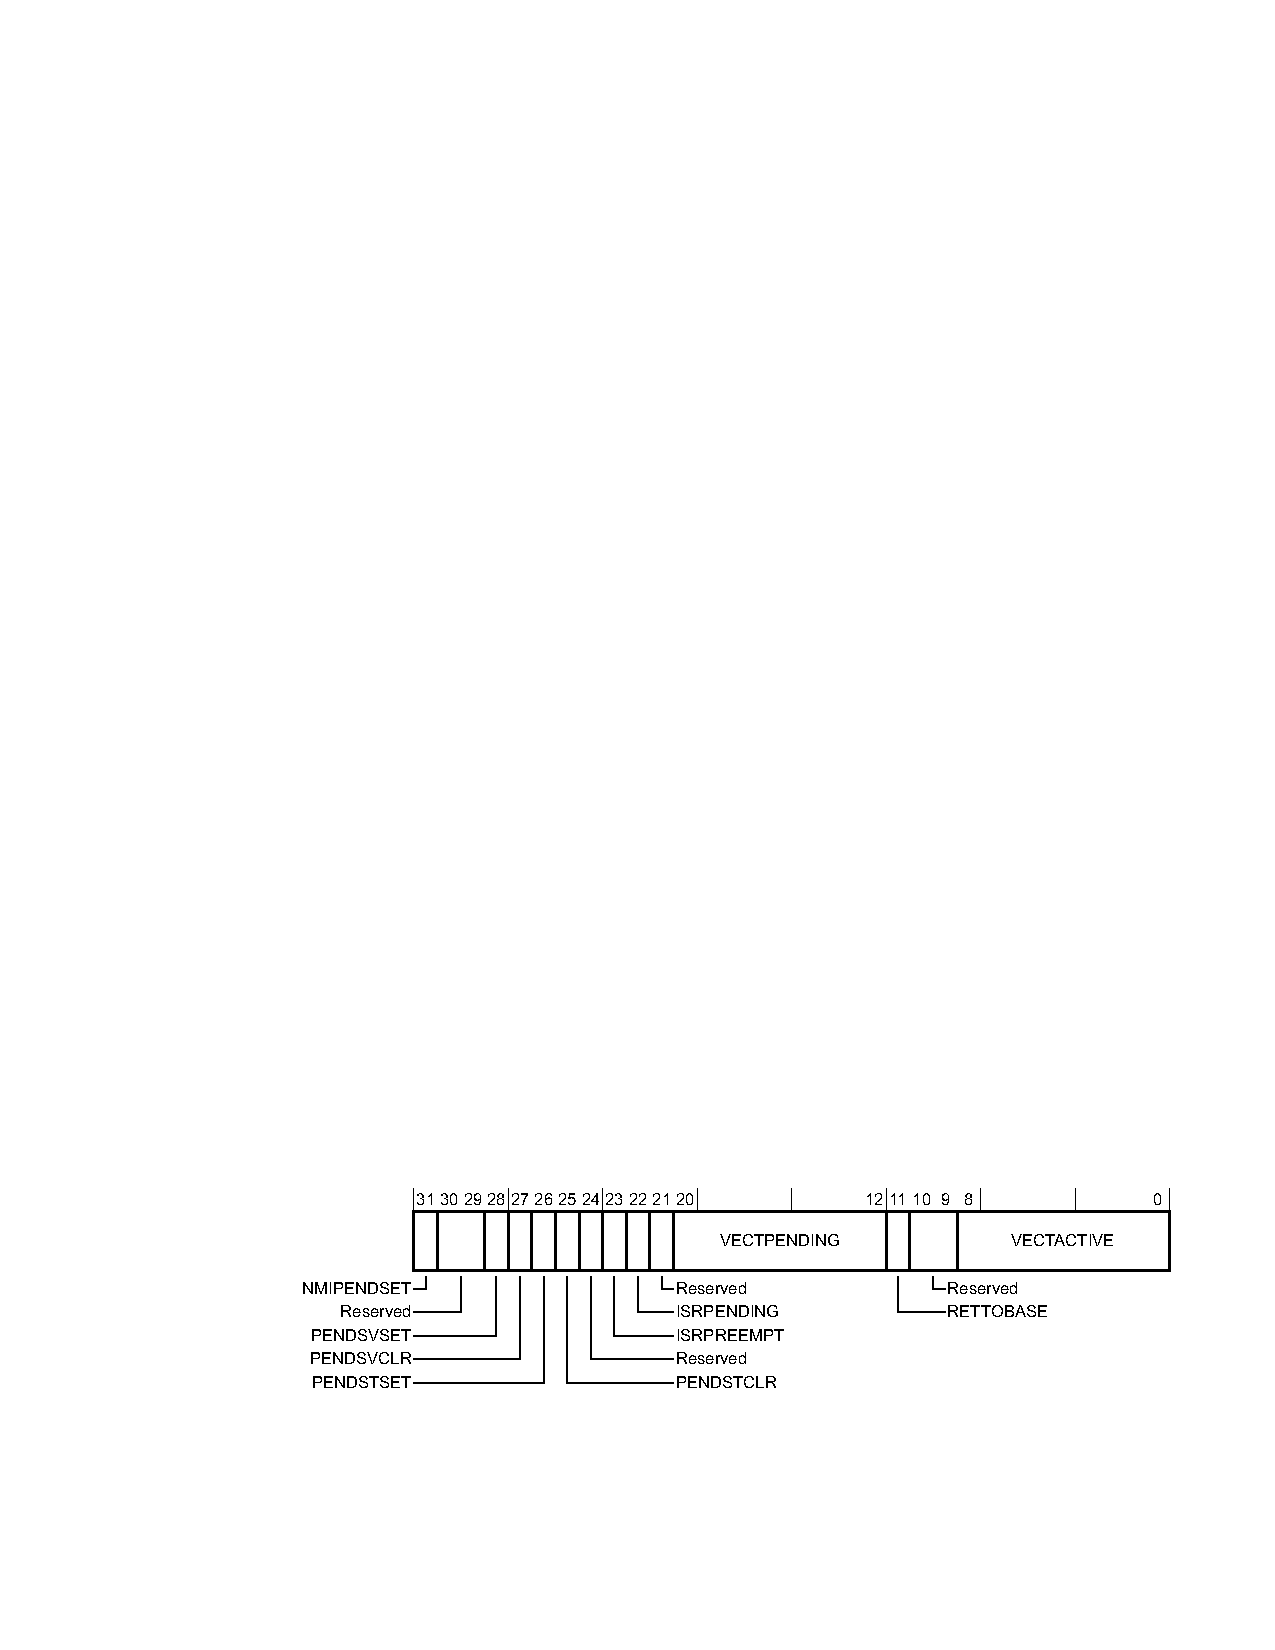
\includegraphics[width=14cm]{chapitres/icsr-armv7m.pdf}
\caption{Registre de contrôle \texttt{ICSR} intégré dans l'ARMv7}
\labelFigure{definitionICSR}
\ligne
\end{figure}




\section{Simple déclaration d'un registre}
Pour déclarer le registre \texttt{ICSR} (\refFigure{}{definitionICSR}), on écrira simplement :
\begin{PLM}
register ICSR at 0xE000_ED04 $uint32
\end{PLM}

Le type \plm+$uint32+ qui est mentionné signifie que les valeurs écrites et lues de ce registre sont des entiers non signés de 32 bits. Tout type entier, signé ou non signé est autorisé.

Pour lire ou écrire ce registre, on le nomme comme s'il s'agissait d'une simple variable. Par exemple, pour activer l'interruption \texttt{PendSV}, il faut mettre à $1$ le bit \texttt{PENDSVSET}. On écrit donc :
\begin{PLM}
ICSR = 1 << 28
\end{PLM}

Si on voulait activer simultanément les interruptions \texttt{PendSV} et \texttt{SysTick}, il faut mettre à $1$ les bits \texttt{PENDSVSET} et \texttt{PENDSTSET}. On écrit donc :
\begin{PLM}
ICSR = (1 << 28) | (1 << 26)
\end{PLM}

Pour savoir si le bit \texttt{RETTOBASE} est activé, on écrit :
\begin{PLM}
let RETTOBASEActif $bool = (ICSR & (1 << 11)) != 0
\end{PLM}

Pour accéder à la valeur du champ \texttt{VECTPENDING}, on réalise un masquage :
\begin{PLM}
let vectPending $uint32 = ICSR & 0x1F_F000
\end{PLM}
 

Et si on veut la valeur de champ justifiée à droite :
\begin{PLM}
let vectPending $uint32 = (ICSR & 0x1F_F000) >> 12
\end{PLM}
 
Ces écritures peuvent être rendues plus intelligibles en précisant la composition du registre \texttt{ICSR} dans sa déclaration. C'est ce qui va être réalisé dans la section suivante.


\sectionLabel{Déclaration d'un registre et de ses champs}{declarationRegistreEtChamps}

Lors de la déclaration d'un registre, il est possible de préciser la composition de ses champs entiers et booléens :
\begin{PLM}
register ICSR at 0xE000_ED04 $uint32 {
  NMIPENDSET, 2, PENDSVSET, PENDSVCLR, PENDSTSET, PENDSTCLR, 1,
  ISRPREEMPT, ISRPENDING, 1, VECTPENDING[9], RETTOBASE, 2, VECTACTIVE[9]
}
\end{PLM}

Entre accolades, trois définitions différentes peuvent apparaître :
\begin{itemize}
\item un nombre indique le nombre de bits consécutifs inutilisés ;
\item un identificateur (par exemple \texttt{NMIPENDSET}) nomme un champ booléen ;
\item un identificateur suivi d'un nombre entre crochets (par exemple \texttt{VECTPENDING[9]}) nomme un champ entier constitué du nombre indiqué de bits consécutifs.
\end{itemize}

La description commence par le bit le plus significatif : comme le type du registre est \plm+$uint32+ (entier non signé sur 32 bits), le premier bit nommé \texttt{NMIPENDSET} porte le n°31, \texttt{PENDSVSET} le n°28, ...

Cette écriture n'est autorisée que si le type nommé (ici \plm+$uint32+) est une type entier non signé. Les types signés (\plm+$int32+, ...) sont interdits. Le compilateur vérifie que la description des champs définit exactement le nombre de bits du type nommé, ici les 32 bits du type \plm+$uint32+.










\subsection{Accès en lecture aux champs booléens}
Pour accéder à la valeur d'un champ, on utilise la notation pointée en nommant ce champ :
\begin{PLM}
let x $uint32 = ICSR.ISRPENDING // 0 ou 2**22
\end{PLM}
Ceci effectue simplement un masquage de façon à isoler le bit demandé. Aucun décalage n'est réalisé. Comme le bit \texttt{ISRPENDING} est le 22\up{e}, le résultat est $0$ ou $2^{22}$.

Si l'on veut obtenir un résultat justifié à droite, on utilise en plus l'accesseur \plm+.shift+ :
\begin{PLM}
let x $uint32 = ICSR.ISRPENDING.shift // 0 ou 1
\end{PLM}

L'accesseur  \plm+.bool+ permet d'obtenir une valeur booléenne correspondant à la valeur d'un bit d'un registre :
\begin{PLM}
let x $bool = ICSR.ISRPENDING.bool // false ou true
\end{PLM}











\subsection{Accès en lecture aux champs entiers}

Comme pour un champ booléen, l'accès à un champ entier s'effectue par la notation pointée \plm+.+. Par exemple :
\begin{PLM}
let x $uint32 = ICSR.VECTPENDING // (0 à 2**9-1) << 12
\end{PLM}

\plm+ICSR.VECTPENDING+ applique un masquage de la valeur de \plm+ICSR+ pour ne conserver que les bits correspondants au champ \plm+VECTPENDING+. Aucun décalage n'est effectué.


Pour obtenir une valeur justifiée à droite, on ajoute l'accesseur \plm+.shift+ :
\begin{PLM}
let x $uint32 = ICSR.VECTPENDING.shift // Entre 0 et 2**9-1
\end{PLM}

La valeur renvoyée est alors comprise en $0$ et $2^9-1$.



\subsection{Constantes associées aux champs booléens}

Le délimiteur \plm+::+ permet de définir des constantes correspondant aux bits d'un registre. Par exemple, pour activer l'interruption \texttt{PendSV}, il faut mettre à $1$ le bit \texttt{PENDSVSET}. On écrit donc :
\begin{PLM}
ICSR = ICSR::PENDSVSET
\end{PLM}

La constante \plm+ICSR::PENDSVSET+ a le type du registre \plm+ICSR+, c'est-à-dire \plm+$uint32+.

De façon analogue, si on voulait activer simultanément les interruptions \texttt{PendSV} et \texttt{SysTick}, il faut mettre à $1$ les bits \texttt{PENDSVSET} et \texttt{PENDSTSET}. On écrit donc :
\begin{PLM}
ICSR = ICSR::PENDSVSET | ICSR::PENDSTSET
\end{PLM}






\subsectionLabel{Expressions associées aux champs entiers}{constructionChampEntierRegistre}

Le délimiteur \plm+::+ permet de simplifier la composition d'une valeur correspondant à un champ entier. Par exemple :

\begin{PLM}
let y $uint32 = ICSR::VECTPENDING (x) // x : expression entière non signée
\end{PLM}

Le champ \texttt{VECTPENDING} est un champ de 9 bits, il peut donc accepter une valeur entière entre $0$ et $511$. L'expression \plm+x+ doit être de type entier non signé. Plusieurs cas sont à considérer :
\begin{itemize}
\item si \plm+x+ est une expression statique, alors le compilateur vérifie que sa valeur est comprise entre $0$ et $511$ (un message d'erreur de compilation est émis dans le cas contraire) ; l'expression \plm+ICSR::VECTPENDING (x)+ est alors aussi une expression statique ;
\item si \plm+x+ est une expression non calculable statiquement :
  \begin{itemize}
  \item si \plm+x+ est du type \plm+$uint8+, alors toute valeur de \plm+x+ est acceptable : le code engendré se borne à faire le décalage à gauche de la valeur de \plm+x+ ;
  \item sinon, une assertion (code : voir \refTableauPage{tableauCodePanique}) est engendrée ; la valeur de \plm+x+ est ensuite masquée pour pallier un éventuel débordement, puis décalée. 
  \end{itemize}
\end{itemize}

D'une manière générale, si \plm+x+ n'est pas calculable statiquement, le code engendré ne comprendra pas d'assertion si le nombre de bits du champ est supérieur ou égal au nombre de bits du type entier de l'expression.





\subsection{Masques associés aux champs entiers}

Le délimiteur \plm+::+ permet de simplifier la composition d'un masque correspondant à un champ entier. Par exemple :

\begin{PLM}
let y $uint32 = ICSR::VECTPENDING // y vaut 0x1F_F000
\end{PLM}

Le champ \texttt{VECTPENDING} est un champ de 9 bits commençant au bit 12. La valeur du masque \plm+ICSR::VECTPENDING+ est donc $(2^9 - 1)^{12}$, soit \texttt{0x1F\_F000}.

Les masques ainsi obtenus sont des expressions statiques.









\sectionLabel{Attribut \texttt{@ro}}{attributRo}\index{"@ro}
La déclaration d'un registre accepte l'attribut \plm+@ro+, qui signifie qu'il est en lecture seule. Par exemple :
\begin{PLM}
register SYST_CALIB @ro at 0xE000_E01C $uint32
\end{PLM}

Toute tentative de faire figurer ce registre dans une construction qui provoque une écriture de celui-ci entraîne l'apparition d'une erreur de compilation.


\section{Déclaration de plusieurs registres}

Il est possible de regrouper les déclarations de registres partageant la même décomposition de leur champs. Par exemple, pour les registres \texttt{PORT$n$\_PCR$m$} du \texttt{mk20dx256} (seule la déclaration de deux premiers registres est montrée) :

\begin{PLM}
register
  PORTA_PCR0 at 0x4004_9000
  PORTA_PCR1 at 0x4004_9004
$uint32 {
  7, isf, 4, irqc[4], lk, 4, mux[3], 1, dse, ode, pfe, 1, sre, pe, ps
}
\end{PLM}












\section{Restrictions d'usage des registres}
\index{Parametre effectif@Paramètre effectif!Registre}

Un registre ne peut pas :
\begin{itemize}
  \item apparaître comme paramètre effectif en entrée d'une procédure ;
  \item apparaître comme paramètre effectif en sortie/entrée d'une procédure.
\end{itemize}

Prenons un exemple ; la procédure \texttt{uneProcedure} présente un argument formel en sortie, et on suppose que \texttt{REGISTRE} est un registre de type \plm!$uint32! :
\begin{PLM}
proc uneProcedure `user (!outValue $uint32) {
  outValue = 5
}
\end{PLM}

L'écriture suivante est correcte (écriture du registre) :
\begin{PLM}
proc autreProcedure `user () {
  REGISTRE = 10 // Ok
}
\end{PLM}


Par contre, l'écriture suivante est rejetée par le compilateur (passage d'un registre comme paramètre effectif en entrée) :
\begin{PLM}
proc autreProcedure `user () {
  uneProcedure (?REGISTRE) // Erreur, registre comme paramètre
                           // effectif en entrée
}
\end{PLM}



%!TEX encoding = UTF-8 Unicode
%!TEX root = ../doc-plm.tex





\chapter{Déclaration des constantes globales}

Les constantes peuvent être déclarées en deux endroits :
\begin{itemize}
  \item en dehors de toute routine : c'est une constante globale (voir ci-après) ;
  \item parmi les instructions d'une routine : c'est une constante locale à la routine (voir \refSectionPage{declarationConstanteLocale}).
\end{itemize}




\sectionLabel{Déclaration d'une constante globale}{declarationConstanteGlobale}\index{Constante!globale}

La déclaration d'une constante globale est la suivante :

\begin{PLM}
let nom : Type = expression_statique
\end{PLM}

Où :
\begin{itemize}
  \item \plm=nom= est le nom de la constante globale ;
  \item \plm=Type= est le nom du type de la constante globale ;
  \item \plm=expression_statique= est l'expression qui fournit la valeur de cette constante~; cette expression est calculée lors de la compilation.
\end{itemize}

La portée d'une constante globale est le programme dans son intégralité : peut importe le fichier et la ligne où elle est déclarée.

L'\plm=expression_statique= ne peut pas nommer une autre constante globale, ni une variable globale. 


%!TEX encoding = UTF-8 Unicode
%!TEX root = ../doc-plm.tex





\chapter{Variables globales}

Une variable est dite \emph{globale} si elle est déclarée en dehors de toute routine, tâche, module.


%Les variables peuvent être déclarées en deux endroits~:
%\begin{itemize}
%  \item en dehors de toute routine~: c'est une variable globale (voir ci-après) ;
%  \item parmi les instructions d'une routine~: c'est une variable locale à la routine (voir \refSectionPage{declarationVariableLocale}).
%\end{itemize}
%




\sectionLabel{Déclaration d'une variable globale}{declarationVariableGlobale}\index{Variable!globale}

La déclaration d'une variable globale est la suivante~:

\begin{PLM}
var nom $type = expression_statique
\end{PLM}

Où :
\begin{itemize}
  \item \plm=nom= est le nom de la variable globale ;
  \item \plm=$type= est le nom du type de la variable globale ;
  \item \plm=expression_statique= est l'expression qui fournit la valeur initiale de cette variable ; cette expression est calculée lors de la compilation.
\end{itemize}

L'\plm=expression_statique= est obligatoire ; si la valeur de celle-ci revient à un zéro binaire, la variable est placée dans une section « \texttt{.bss.*} », de façon à être initialisée au début de l'exécution (\refSectionPage{sequenceDemarrage}).

La portée d'une variable globale est le programme dans son intégralité~: peu importe où est déclarée la variable.

% Toutefois, seules les routines explicitement autorisées dans peuvent y accéder.
%
%L'\plm=expression_statique= peut utiliser la valeur des constantes globales~: le compilateur évalue les constantes globales avant d'évaluer les valeurs initiales des variables globales. Par contre, \plm=expression_statique= ne peut pas utiliser les valeurs d'une autre variable globale.
%
%Par exemple, voici comment on peut implémenter une variable globale \texttt{gCompteur}, incrémentée par la routine d'interruption \texttt{timerHandler}, et écrire un service d'attente de délai \texttt{wait} avec une boucle d'attente active~:
%
%\begin{PLM}
%var gCompteur $uint32 = 0 {
%  @rw func timerHandler // Ne pas faire figurer
%  func waitMS           // la liste des arguments
%}
%
%func timerHandler isr () {
%  gCompteur +%= 1
%}
%
%func wait user (?inDuration $uint32) {
%  let deadline = gCompteur + inDuration
%  while gCompteur < deadline do
%  end
%}
%\end{PLM}
%
%Note~: si une variable globale est accédée par des routines appartenant à plusieurs modes, le compilateur ajoute le qualificatif \texttt{volatile}\index{volatile@\texttt{volatile}} dans le code engendré pour déclarer cette variable. C'est le cas de l'exemple ci-dessus, la variable \texttt{gCompteur} pouvant être accédée dans les modes \plm=isr= et \plm=user=.
%
%
%Les routines d'initialisation (\refSectionPage{initRoutine})\index{init@\plm=init=!Routine} et les routines de panique (\refSubsectionPage{routinesPanique})\index{Routine!panique \plm=panic=}
% doivent de même être déclarées pour pouvoir accéder à une variable globale (et avec l'attribut \plm=@rw= si on veut l'accès en écriture). Par exemple~:
%\begin{PLM}
%var gCompteur $uint32 = 0 {
%  @rw init 112
%  @rw func panic loop 179
%}
%
%func init 112 {
%  gCompteur = 10
%}
%
%func panic loop 179 {
%  gCompteur = 100
%}
%\end{PLM}
%
%
%\sectionLabel{Déclarations des routines autorisées}{DecRoutinesAutoriseesVarGlobale}
%
%Dans la déclaration d'une variable globale, \plm=en_tetes_routines_autorisees= liste l'ensemble des routines pouvant accédéer à la variable globale. Cette liste doit être non vide. On peut ainsi autoriser l'accès à~:
%\begin{itemize}
%  \item une routine d'initialisation (\plm!init!) ;
%  \item une fonction (\plm!func!) ;
%  \item une section (\plm!section!) ;
%  \item une routine de panique (\plm!func panic!) ;
%  \item une fonction de type (\plm!func!).
%\end{itemize}
%
%Le \refTableauPage{DecRoutinesAutoriseesAccesVarGlobale} résume les déclarations des routines autorisées. Par défaut, seul l'accès en lecture est permis. L'attribut \plm!@rw! permet d'autoriser pour une routine l'accès en écriture, sauf pour les fonctions ou cet attribut est interdit.
%
%Le compilateur interdit l'accès des routines \plm+boot+ aux variables globales\footnote{En effet, comme les routines \texttt{boot} sont exécutées avant l'initialisation des variables globales, le comportement à l'exécution serait indéfini.}.
%
%\begin{table}[t]
%\centering
%\begin{tabular}{lp{5cm}l}
%  \textbf{Déclaration} & \textbf{Routine autorisée} & \textbf{Accés en écriture} \\
%  \plm=init priorite= & Routine d'initialisation de priorité \plm=priorite= & Nécessite \plm!@rw! \\
%  \plm=func nom= & Fonction \plm!nom! & Jamais \\
%  \plm=section nom= & Section \plm!nom! & Nécessite \plm!@rw! \\
%  \plm=func panic nom prorite= & Routine de panique \plm!nom! de priorité \plm=priorite= & Nécessite \plm!@rw! \\
%  \plm=func $type nom= & Procédure \plm!nom! du type \plm!$type! & Nécessite \plm!@rw! \\
%  \plm=func $type nom= & Fonction \plm!nom! du type \plm!$type! & Jamais \\
%\end{tabular}
%\caption{Déclaration des routines autorisées}
%\labelTableau{DecRoutinesAutoriseesAccesVarGlobale}
%\ligne
%\end{table}













\sectionLabel{Restrictions d'usage des variables globales}{restrictionUsageVariableGlobale}

La concurrence impose des restrictions sur l'usage des variables globales. Pour les illustrer, nous prenons l'exemple d'une variable globale \plm+gVariable+, de type \plm=$s= :

\begin{PLM}
var gVariable = $s ()

struct $s {
  var mX $uint32 = 0 ;
  var mY $uint32 = 0 ;
  
  func increment @mutating @access () {
    mX += 1
    mY += 1
  }

  func section atomicIncrement @mutating @access () {
    mX += 1
    mY += 1
  }

  func indirectIncrement @mutating () {
    self.atomicIncrement ()
  }
}
\end{PLM}

Pour mémoire (§), l'attribut \plm=@access= signifie que la méthode accède {\bf directement} aux propriétés : c'est le cas de \plm=increment= et de \plm=atomicIncrement=. L'attribut \plm=@mutating= signifie que la méthode modifie la valeur des propriétés, directement (si \plm=@access= est présent), ou indrectement (pas d'attribut \plm=@access=), comme c'est le cas de la méthode \plm=indirectIncrement=.

\subsection{Accès à une variable globale}


Afin de préciser ces règles, il convient de rappeler les différents types d'accès à une variable :
\begin{enumerate}[label=(\arabic*)]
  \item accès en lecture (par exemple \plm+var u = gVariable+) ;
  \item accès en écriture (par exemple \plm+gVariable = u+) ;
  \item accès en lecture / écriture (par exemple \plm!gVariable += u!) ;
  \item appel d'une méthode, par exemple \plm+gVariable.increment ()+.
\end{enumerate}

L'accès en lecture (1), en écriture (2), en lecture / écriture (3) est interdite à une routine s'exécutant dans le mode \plm=user=. Il en est de même pour les fonctions «~universelles~» (\refSubsectionPage{fonctionUniverselle}) : leur mode d'exécution n'étant pas fixé à la compilation, il se peut qu'elles s'exécutent en mode \plm+user+.

Le cas (4) est plus difficile à appréhender. Si la méthode est déclarée en mode privilégié, l'appel est possible sans restriction, comme par exemple \plm+gVariable.atomicIncrement ()+. Par contre, \plm+gVariable.increment ()+ est interdit, et détecté comme une erreur par le compilateur : en effet, appelé en mode \plm=user=, l'incrémentation des propriétés ne serait pas atomique. L'appel \plm+gVariable.indirectIncrement ()+ est autorisé, puisque l'incrémentation est réalisé par une routine en mode privilégié.

En résumé :
\begin{itemize}
  \item l'appel d'une méthode privilégiée d'une variable globale est autorisée ;
  \item l'appel d'une méthode «~universelle~» ou \plm=user= d'une variable globale est autorisée, sous réserve que cette méthode n'ait pas l'attribut \plm=@access=.
\end{itemize}








\subsection{Variable globale comme paramètre effectif}

Une variable globale ne peut pas~:\index{Parametre effectif@Paramètre effectif!Variable globale}

\begin{itemize}
  \item apparaître comme paramètre effectif en entrée d'une fonction ;
  \item apparaître comme paramètre effectif en sortie/entrée d'une fonction.
\end{itemize}

Par contre, sous certaines conditions, une variable globale peut apparaître en paramètre effectif de sortie : la routine appelante doit être privilégiée. La transmission d'un paramètre effectif en sortie implique une copie, or en mode \plm=user=, celle-ci n'est pas atomique.



%!TEX encoding = UTF-8 Unicode
%!TEX root = ../doc-plm.tex





\chapterLabel{Modes d'exécution}{chapitreModesExecution}

\colorbox{red}{Doc à écrire.}

%!TEX encoding = UTF-8 Unicode
%!TEX root = ../doc-plm.tex





\chapter{Routines}

Le langage définit plusieurs natures de sous-programmes :
\begin{itemize}
  \item les \emph{procédures}, dont l'appel est une instruction ;
  \item les \emph{fonctions}, dont l'appel apparaît dans une expression ;
  \item les \emph{boot routines}, exécutées une fois avant l'initialisation des variables globales ;
  \item les \emph{init routines}, exécutées une fois après l'initialisation des variables globales ;
  \item les \emph{routines d'exception}, exécutées lors d'une exception (\refSectionPage{routineException}).
\end{itemize}

Les \emph{routines}\index{Routine} se distinguent des \emph{procédures} et des \emph{fonctions} par le fait qu'elles n'ont pas d'arguments formels explicites, et qu'elles ne peuvent pas être appelées explicitement.









\sectionLabel{\texttt{boot} routines}{bootRoutine}
\index{boot@\plm=boot=!Routine}
\index{Routine!boot@\plm=boot=}

Une routine \plm=boot= est exécutée une et une seule fois, lors du démarrage du micro-contrôleur, avant que les variables globales ne soient initialisées. Elle a la syntaxe suivante :
\begin{PLM}
boot priorite {
  liste_instructions
}
\end{PLM}
Où \plm=priorite= est la priorité de la routine. C'est une constante entière entre $0$ et $2^{64}-1$. Les routines \plm=boot= sont exécutées dans l'ordre des priorités croissantes. Le compilateur vérifie que deux routines \plm=boot= n'ont pas la même priorité.

Les routines \plm=boot= s'exécutent dans le mode \plm=`boot=.\index{\`boot}

Comme les routines \plm=boot= s'exécutent avant que les variables globales soient initialisées, l'accès aux variables globales y est interdit. L'interdiction est mise en place de la façon suivante : il n'est pas possible d'associer une routine \plm=`boot= à une variable globale lors de sa déclaration (\refSectionPage{declarationVariableGlobale}).

Par contre, l'accès aux registres de contrôle est autorisé dans une routine \plm=boot= (d'ailleurs, elle sert à cela : configurer le micro-contrôleur au démarrage).







\sectionLabel{\texttt{init} routines}{initRoutine}
\index{init@\plm=init=!Routine}
\index{Routine!init@\plm=init=}

Une routine \plm=init= est exécutée une et une seule fois, lors du démarrage du micro-contrôleur, après l'initialisation des variables globales. Elle a la syntaxe suivante :
\begin{PLM}
init priorite {
  liste_instructions
}
\end{PLM}
Où \plm=priorite= est la priorité de la routine. C'est une constante entière entre $0$ et $2^{64}-1$. Les routines \plm=init= sont exécutées dans l'ordre des priorités croissantes. Le compilateur vérifie que deux routines \plm=init= n'ont pas la même priorité.

Les routines \plm=init= s'exécutent dans le mode \plm=`init=.\index{\`init}

Comme les routines \plm=init= s'exécutent après l'initialisation des variables globales, l'accès aux variables globales y est autorisé, du moment que la variable globale cite le mode \plm=`init= dans sa déclaration (\refSectionPage{declarationVariableGlobale}).






\sectionLabel{Arguments formels, paramètres effectifs, sélecteurs}{argumentFormel}
\index{Argument formel}
\index{Parametre effectif@Paramètre effectif}
\index{Selecteur@Sélecteur}

Il existe trois natures d'arguments formels : \emph{entrée}, \emph{sortie} et \emph{entrée / sortie}, décrits dans le \refTableau{argumentsFormels}. Un sélecteur peut être \emph{anonyme} (par exemple \plm+?+ pour un paramètre formel en entrée), ou comporter un nom (le nom « \texttt{nom} » pour \plm+?nom:+).

Une procédure déclare zéro, un ou plusieurs arguments formels qui peuvent être en \emph{entrée}, en \emph{sortie} ou en \emph{entrée/sortie}. Une fonction déclare zéro, un ou plusieurs arguments formels en \emph{entrée}.

La syntaxe des différents arguments formels et de leur paramètre effectif est résumée dans le \refTableau{argumentsFormelsParametresEffectifs}. 

\begin{table}[t]
  \centering
  \begin{tabular}{lp{6.5cm}l}
    \textbf{Argument formel} & \textbf{Transfert d'information} & \textbf{Sélecteur} \\
    Entrée & Lors de l'appel, de l'appelant vers l'appelé & \plm+?+ ou \plm+?selecteur:+\\
    Sortie & Lors du retour, de l'appelé vers l'appelant & \plm+!+ ou \plm+!selecteur:+\\
    Entrée / sortie & Lors de l'appel, de l'appelant vers l'appelé, et lors du retour, de l'appelé vers l'appelant & \plm+?!+ ou \plm+?!selecteur:+\\
  \end{tabular}
  \caption{Arguments formels}
  \labelTableau{argumentsFormels}
  \ligne
\end{table}



\begin{table}[t]
  \centering
  \begin{tabular}{llll}
    \textbf{Argument formel} & \textbf{Sélecteur} & \textbf{Paramètre effectif} & \textbf{Sélecteur} \\
    Entrée & \plm+?+         & Sortie & \plm+!expression+ \\
           & \plm+?selecteur:+ & & \plm+!selecteur:expression+ \\
    Sortie & \plm+!+         & Entrée & \plm+?variable+ \\
           & \plm+!selecteur:+ & & \plm+?selecteur:variable+ \\
    Entrée/sortie & \plm+?!+         & Sortie/entrée & \plm+!?variable+ \\
           & \plm+?!selecteur:+ & & \plm+!?selecteur:variable+ \\
  \end{tabular}
  \caption{Argument formel et paramètre effectif}
  \labelTableau{argumentsFormelsParametresEffectifs}
  \ligne
\end{table}







\section{Procédure}


\subsectionLabel{Déclaration d'une procédure}{declarationProcedure}\index{Procedure@Procédure}

La déclaration d'une procédure est la suivante :
\begin{PLM}
proc nom `mode1 `mode2 @attribut1 @attribut2 (arguments_formels) {
  liste_instructions
}
\end{PLM}
Où :
\begin{itemize}
  \item \plm=nom= est le nom de la procédure ;
  \item \plm=`mode1= \plm=`mode2= est la liste non vide de l'ensemble des modes associés à la procédure ;
  \item \plm=@attribut1= \plm=@attribut2= est une liste éventuellement vide d'attributs associés à la procédure.
\end{itemize}

Par exemple :

\begin{PLM}
proc setup `user () {
}
\end{PLM}

Ceci définit la procédure \plm=setup=, sans argument, sans attribut, appelable uniquement en mode \plm=`user=.

\begin{PLM}
proc goto `user @noWarningIfUnused (
  ?line:inLine $uint32
  ?column:inColumn $uint8) {
}
\end{PLM}

Ceci définit la procédure \plm=goto=, appelable uniquement en mode \plm=`user=, avec deux arguments formels en entrée. L'attribut \plm+@noWarningIfUnused+ signifie qu'aucune alerte n'est émise si la procédure n'est pas utilisée.







\subsectionLabel{Attribut \texttt{@noWarningIfUnused}}{attributNoWarningIfUnused}\index{"@noWarningIfUnused}

L'attribut \plm+@noWarningIfUnused+ signifie qu'aucune alerte n'est émise si la procédure n'est pas utilisée.



\subsectionLabel{Attribut \texttt{@weak}}{attributWeak}\index{"@weak}

L'attribut \plm+@weak+ signifie que la routine peut être redéfinie par une routine de même nom, avec les mêmes arguments formels, les mêmes modes. Les fichiers de définition de cible utilisent cette possibilité pour définir des routines par défaut.

Par exemple, la cible \texttt{teensy-3-1-it} définit cette routine d'interruption (voir le deuxième exemple du tutorial, \refSectionPage{deuxiemeExemple}) :

\begin{PLM}
proc systickHandler `isr @weak () {
}
\end{PLM}

Par défaut, la routine d'interruption \plm+systickHandler+ est donc définie, vide. Le programme d'exemple définit cette routine :

\begin{PLM}
proc systickHandler `isr () {
  gUpTimeMS ++
}
\end{PLM}

Comme cette nouvelle routine a le même nom, les mêmes arguments formels et le même mode que la routine marquée \plm+@weak+, elle est utilisée à la place de celle-ci.






\subsectionLabel{Attribut \texttt{@nullWhenPanicDisabled}}{attributNullOnNoException}\index{"@nullWhenPanicDisabled}

L'attribut \plm+@nullWhenPanicDisabled+ signifie que la procédure est éliminée si le projet est compilé avec les exceptions désactivées (option \OPTION{-{}-no-panic-generation}, \refSectionPage{optionCodeEngendre}). Les références à cette routine sont alors remplacées par la valeur zéro.

Cette option est à utiliser en toute connaissance de cause. Elle sert à éliminer les routines d'interruption qui ne sont pas utilisées dans un projet.

Par exemple, une routine d'interruption par défaut est déclarée par la cible :

\begin{PLM}
proc svcHandler `isr @nullWhenPanicDisabled @weak () {
  panic 11
}
\end{PLM}

Si cette routine n'est pas redéfinie par une routine de même nom, et que le programme est compilé avec les exception activées, alors l'occurrence de l'interruption déclenchera l'exception n°11.

Si cette routine n'est pas redéfinie par une routine de même nom, et que le programme est compilé avec les exception désactivées, alors l'attribut \plm+@nullWhenPanicDisabled+ fera que la routine sera éliminée de la génération de code, et l'entrée correspondante de la table des interruptions sera mise à zéro. Cela permet de ne pas engendrer de code inutile dans cette situation.

 





\subsectionLabel{Procédures requises}{procedureRequise}

La déclaration \plm+required proc+ permet de signifier au compilateur qu'une procédure doit être définie, soit par la cible, soit par le programme utilisateur.

Cette déclaration est la suivante :
\begin{PLM}
required proc nom `mode1 `mode2 @attribut1 @attribut2 (arguments_formels)
\end{PLM}

Elle consiste à la déclaration de l'en-tête d'une procédure (voir \refSubsectionPage{declarationProcedure}), précédée par le mot réservée \plm+required+.

Par exemple, la cible \texttt{teensy-3-1-it} comporte ces deux déclarations :

\begin{PLM}
required proc setup `user ()
required proc loop `user ()
\end{PLM}

Ceci impose au programme utilisateur de définir ces deux procédures.









\section{Fonctions}

\colorbox{red}{À définir}







\section{Routines utiles}

Le compilateur élimine les procédures qui ne sont jamais appelées, en calculant le graphe des appels. Les racines de ce graphe sont les procédures requises (\refSubsectionPage{procedureRequise}), les routines \plm=boot=, \plm=init= et \plm=exception=. Les procédures et fonctions inatteignables sont éliminées, avec ou sans message d'alerte (\refSubsectionPage{attributNoWarningIfUnused}).











\sectionLabel{Récursivité}{routinesRecursives}\index{Routines!recursives@récursives}

Par défaut, le compilateur émet un message d'erreur si une ou plusieurs routines récursives sont détectées. L'option \OPTION{-{}-do-not-detect-recursive-calls} (\refSectionPage{optionCodeEngendre}) permet d'inhiber cette recherche.

L'option \OPTION{-{}-routine-invocation-graph} permet d'obtenir un fichier contenant le graphe d'invocation, qui peut être affiché par le logiciel \texttt{graphviz}\index{graphviz}. Si le fichier source est \texttt{source.plm}, le fichier engendré s'appelle \texttt{source.subprogramInvocation.dot}.


%!TEX encoding = UTF-8 Unicode
%!TEX root = ../doc-plm.tex





\chapter{Expressions}


\begin{table}[ht]
\centering
\begin{tabular}{llll}
  \textbf{Priorité} & \textbf{Opérateur} & \textbf{Commentaire} & \textbf{Lien} \\
   0 (plus prioritaire) & \plm+-+, \plm+-%+ & \emph{moins} unaire & \\
   0 & \plm+~+, \plm+not+ & \emph{non} binaire et \emph{non} logique & \\
   1 & \plm=convert= & Conversion &\\
   2 & \plm+*+, \plm+*%+, \plm+/+, \plm+!/+, \plm-%-, \plm-!%- & Multiplication, division, modulo & \\
   3 & \plm-+-, \plm-+%-, \plm+-+, \plm+-%+ & Addition, soustraction & \\
   4 & \plm+<<+, \plm+>>+ & Décalage à gauche et à droite & \\
   5 & \plm+<=+, \plm+<+, \plm+>=+, \plm+>+ & Comparaison & \\
   6 & \plm+==+, \plm+!=+ & Test d'égalité, d'inégalité & \\
   7 & \plm+&+ & \emph{et} binaire & \\
   8 & \plm+^+ & \emph{ou exclusif} binaire & \\
   9 & \plm+|+ & \emph{ou} binaire & \\
   10 & \plm+and+ & \emph{et} logique & \\
   11 & \plm+xor+ & \emph{ou exclusif} logique & \\
   12 (moins prioritaire) & \plm+or+ & \emph{ou} logique & \\
\end{tabular}
\caption{Priorité des opérateurs}\index{Operateur@Opérateur!Priorite@Priorité}
\labelTableau{tableauPrioriteOperateurs}
\end{table}

%!TEX encoding = UTF-8 Unicode
%!TEX root = ../doc-plm.tex





\chapter{Instructions}





\sectionLabel{Déclaration d'une variable locale}{declarationVariableLocale}\index{Variable!locale}

La déclaration d'une variable locale peut prendre plusieurs formes, suivant que la variable est initialisée ou non.

\subsection{Déclaration d'une variable locale initialisée}

\begin{PLM}
var nom : Type = expression
\end{PLM}

Où :
\begin{itemize}
  \item \plm=nom= est le nom de la variable locale ;
  \item \plm=Type= est le nom du type de la variable globale ;
  \item \plm=expression= est l'expression qui fournit la valeur initiale de cette variable ; cette expression peut être statique ou non.
\end{itemize}

L'annotation de type peut être omise ; la variable a alors le type de l'expression qui l'initialise :
\begin{PLM}
var nom = expression
\end{PLM}


\subsection{Déclaration d'une variable locale non initialisée}
\begin{PLM}
var nom : Type
\end{PLM}
Où :
\begin{itemize}
  \item \plm=nom= est le nom de la variable locale ;
  \item \plm=Type= est le nom du type de la variable globale.
\end{itemize}

Le compilateur garantit qu'aucune lecture n'est faite avant que la variable reçoive une valeur.










\sectionLabel{Déclaration d'une constante locale}{declarationConstanteLocale}\index{Constante!locale}

La déclaration d'une constante locale apparaît dans une liste d'instructions et sa syntaxe est la suivante :

\begin{PLM}
let nom : Type = expression
\end{PLM}

Où :
\begin{itemize}
  \item \plm=nom= est le nom de la constante globale ;
  \item \plm=Type= est le nom du type de la constante globale ;
  \item \plm=expression= est l'expression qui fournit la valeur de cette constante ; cette expression est soit calculable statiquement, soit à l'exécution.
\end{itemize}

Il n'y a aucune restriction pour l'\plm=expression= : elle peut nommer constantes locales et globales, variables locales et globales.






\section {Instruction d'affectation}

L'instruction d'affectation est la suivante :

\begin{PLM}
nom = expression
\end{PLM}

Où :
\begin{itemize}
  \item \plm=nom= est le nom d'une variable glogale ou locale, ou le nom d'un registre de contrôle ;
  \item \plm=expression= est l'expression qui fournit la valeur.
\end{itemize}











\sectionLabel{Instructions d'incrémentation et de décrémentation}{instructionIncDec}
\index{Incrementation@Incrémentation!Instruction}
\index{Decrementation@Decrémentation!Instruction}

Les opérateurs postfixés \plm=++= et \plm=--= réalisent respectivement l'incrémentation et la décrémentation de la variable nommée dans l'instruction :
\begin{PLM}
variable ++
\end{PLM}

\plm=++= et \plm=--= engendrent une exception sur dépassement de capacité.

Les opérateurs \plm=&++= et \plm=&--= ignorent le dépassement de capacité.

Les instructions d'incrémentation et de décrémentation de variables entières sont détaillées à la \refSectionPage{incDecEntier}.






\sectionLabel {Opérateurs combinés avec une affectation}{operateursCombinesAffectation}
\index{\&=}
\index{\textbar=}
\index{\^{}=}

\plm!a &= b! est équivalent à \plm!a = a & b!.

\plm!a |= b! est équivalent à \plm!a = a | b!.

\plm!a ^= b! est équivalent à \plm!a = a ^ b!.

Les opérateurs infixes \plm!&=!, \plm!|=! et \plm!^=! sur les entiers sont décrits à la \refSectionPage{operateursCombinesAffectationEntier}.


\sectionLabel{Instruction \texttt{check}}{directiveCheck}\index{check@\plm=check=}

La directive \plm=check= apparaît dans une liste d'instructions et a la syntaxe suivante :
\begin{PLM}
check expression
\end{PLM}

L'\plm=expression= est une expression booléenne calculée statiquement.

Contrairement à l'instruction \plm=assert= (\refSectionPage{instructionAssert}) qui évalue l'expression booléenne à l'exécution, la directive \plm=check= est toujours évaluée à la compilation. Elle permet d'exprimer des assertions qui sont évaluées lors de la compilation.

Aucun code n'est engendré. La directive \plm=check= peut donc apparaître dans des listes d'instructions où les exceptions sont interdites.

Exemples :
\begin{PLM}
check true  // Ok
check false // Erreur, expression fausse
\end{PLM}



\sectionLabel{L'instruction \texttt{assert}}{instructionAssert}\index{assert@\plm=assert=}

L'instruction \plm=assert= a la syntaxe suivante :
\begin{PLM}
assert expression
\end{PLM}

L'\plm=expression= est une expression booléenne non calculable statiquement.

Si le programme est compilé avec les exceptions activées, alors le compilateur engendre le code de calcul de l'expression booléenne. Celle-ci sera calculée à l'exécution. Si le résultat est faux, une exception (dont le code est donné par le \refTableau{tableauCodeExceptions}) est levée.

Si le programme est compilé avec l'option \texttt{-{}-no-exception-generation}, alors aucun code n'est engendré.

Noter que \plm=expression= ne doit pas être calculable statiquement. Si elle est calculable statiquement, il faut utiliser la directive \plm=check=, \refSectionPage{directiveCheck}. Par exemple, le code suivant provoque une erreur de compilation :
\begin{PLM}
assert true // Erreur, l'expression est calculable statiquement
\end{PLM}



\section{L'instruction \texttt{throw}}\index{throw@\plm=throw=}

L'instruction \plm=throw= a la syntaxe suivante :
\begin{PLM}
throw expression
\end{PLM}

L'\plm=expression= est une expression entière, calculée statiquement. Son type est défini pour chaque cible (\refSectionPage{typeLiesException}) et peut être signé (les valeurs négatives sont alors acceptées) ou non signé.

Si le programme est compilé avec les exceptions activées, alors l'exécution de l'instruction \plm=throw= lève une exception dont le code est la valeur de l'\plm=expression=.

Si le programme est compilé avec l'option \texttt{-{}-no-exception-generation}, alors aucun code n'est engendré.




\sectionLabel{Instruction d'appel de procédure}{instructionAppelProc}

\colorbox{red}{À définir}


\section{Instruction \texttt{if}}
\index{if@\plm=if=}

L'instruction \plm=if= a une structure classique, où \plm=condition= est une expression booléenne :
\begin{PLM}
if condition then
  instructions_then
else
  instructions_else
end
\end{PLM}

Le compilateur vérifie que la \plm=condition= n'est pas une expression statique : une erreur de compilation est émise si elle l'est.

La branche \plm=else= est optionnelle :
\begin{PLM}
if condition then
  instructions_then
end
\end{PLM}


Une ou plusieurs branches \plm=elsif= peuvent être ajoutées :
\begin{PLM}
if condition then
  instructions_then
elsif condition2 then
  instructions_elsif
end
\end{PLM}






\section{Instruction \texttt{while}}
\index{if@\plm=while=}

L'instruction \plm=while= permet d'exprimer une répétition, où la \plm=condition= est testée avant l'exécution des instructions de la boucle :
\begin{PLM}
while condition do
  instructions_while
end
\end{PLM}

\plm=condition= est une expression booléenne, qui ne doit pas être statique : une erreur de compilation est émise si elle l'est.


%!TEX encoding = UTF-8 Unicode
%!TEX root = ../doc-plm.tex





\chapter{Directives}


\sectionLabel{Directive \texttt{target}}{directiveTarget}\index{target@\plm=target=}

La directive \plm=target= fixe la cible pour laquelle le code source est compilé. Sa syntaxe est la suivante~:
\begin{PLM}
target "cible"
\end{PLM} 
Où \plm="cible"= est le nom du descriptif de la cible.





\sectionLabel{Directive \texttt{import}}{directiveImport}\index{import@\plm=import=}


La directive \plm=import= permet d'ajouter les définitions contenues dans le fichier texte nommé. Sa syntaxe est la suivante~:
\begin{PLM}
import "chemin.plm"
\end{PLM} 
Où \plm="chemin.plm"= est un chemin (absolu, relatif) vers le fichier à importer.

Importer plusieurs fois le même fichier n'est pas une erreur. Le compilateur garde trace des importations déjà effectuées et ignore les importations des fichiers déjà importés.

L'extension \texttt{.plm} doit être mentionnée dans le chemin.


\sectionLabel{La directive \texttt{check target}}{directiveCheckTarget}\index{check target}

La directive \plm=check target= permet de vérifier l'identité de la cible. Elle est utile pour s'assurer qu'un fichier est acceptable par une cible. À la compilation, toute directive \plm=check target= incorrecte entraîne une erreur.

Par exemple, compiler pour la cible \plm+"teensy-3-1"+ est spécifié par~:

\begin{PLM}
target "teensy-3-1"
\end{PLM}

Si la définition du projet implique d'importer le fichier \plm+"monFichier.plm"+~:

\begin{PLM}
target "teensy-3-1"
import "monFichier.plm"
\end{PLM}

Si le contenu de ce fichier commence par~:
\begin{PLM}
check target "lpc2294"
\end{PLM}

Alors une erreur de compilation apparaît. La directive \plm=check target= doit être~:
\begin{PLM}
check target "teensy-3-1"
\end{PLM}


%!TEX encoding = UTF-8 Unicode
%!TEX root = ../doc-plm.tex





\chapter{Exceptions}


\begin{table}[ht]
\centering
\small
\begin{tabular}{lp{7cm}l}
  \textbf{Numéros} & \textbf{Signification} & \textbf{Lien} \\
  \hline
   < 0 & Exceptions liées aux vecteurs d'interruption & \\
   1 & Dépassement de capacité de l'incrémentation (\plm-++-) & \refSectionPage{instructionIncDec} \\
   2 & Dépassement de capacité de l'incrémentation (\plm+--+) & \refSectionPage{instructionIncDec} \\
   3 & Dépassement de capacité de la négation (\plm+-+) & \refSubsectionPage{negationOvf} \\
   4 & Dépassement de la construction d'un champ entier d'un registre (\plm+registre::champ (...)+) & \refSubsectionPage{constructionChampEntierRegistre}\\
   5 & Dépassement de capacité d'une conversion entre entiers (\plm+\+) & \refSectionPage{operateursInfixArithmétiques} \\
   10 & Dépassement de capacité de l'addition (\plm-+-) &  \refSectionPage{operateursInfixArithmétiques} \\
   11 & Dépassement de capacité de la soustraction (\plm+-+) & \refSectionPage{operateursInfixArithmétiques} \\
   12 & Dépassement de capacité de la multiplication (\plm+*+) & \refSectionPage{operateursInfixArithmétiques} \\
   13 & Dépassement de capacité de la division (\plm+/+) & \refSectionPage{operateursInfixArithmétiques} \\
   14 & Modulo par zéro (\plm+%+) & \refSectionPage{operateursInfixArithmétiques} \\
   20 & Échec de l'instruction \plm+assert+ & \refSectionPage{instructionAssert} \\
\end{tabular}
\caption{Code des exceptions}\index{Exception!Code}
\labelTableau{tableauCodeExceptions}
\end{table}






\sectionLabel{Définition des types liés aux exceptions}{typeLiesException}\index{exception:@\plm=exception:=}

Une exception est caractérisée par trois informations :
\begin{itemize}
  \item son code (\refTableauPage{tableauCodeExceptions}) ;
  \item le nom du fichier source de l'instruction qui a levé l'exception ;
  \item le numéro de ligne du fichier source de l'instruction qui a levé l'exception.
\end{itemize}

Le type du code et du numéro de ligne ne sont pas prédéfinis par le langage. La construction suivante définit ces types :
\begin{PLM}
exception : nomDuTypeDuCode nomDuTypeDuNumeroDeLigne
\end{PLM}

Par exemple, les numéros de code sont des entiers signés 32 bits, et les numéros de ligne des entiers non signés 32 bits :
\begin{PLM}
exception : Int32 UInt32
\end{PLM}

Cette construction doit apparaître exactement une fois. Normalement, c'est le fichier de définition de la cible qui la contient.


\sectionLabel{Routines exécutées lors de l'occurrence d'une exception}{routineException}

\begin{figure}[t]
  \centering
  \small
  \begin{tikzpicture}[
      cloud/.style ={draw=red, thick, ellipse,fill=red!20, minimum height=2em},
      block/.style ={rectangle, draw=blue, thick, fill=green!20, align=center},
      decision/.style={chamfered rectangle, draw=blue, thick, fill=green!20},
      node distance=5mm
    ]
    \node [cloud] (start) {\textsc{Occurrence d'une exception}} ;
    \node [block] (raz) [below=of start] {Masquage des interruptions} ;
    \node [block] (setup) [below=of raz] {Routines \texttt{\bf exception} \texttt{setup}} ;
    \node [block] (loop) [below=of setup] {Routines \texttt{\bf exception} \texttt{loop}} ;

    \draw [-stealth, thick] (start) -- (raz) ;
    \draw [-stealth, thick] (raz) -- (setup) ;
    \draw [-stealth, thick] (setup) -- (loop) ;
    \draw [-stealth, thick] (loop.south) -- +(0, -.25) -- +(2.75, -.25) -- +(2.75, 0.75)-- +(0, 0.75) ;
  \end{tikzpicture}
  \caption{Organigramme de la réponse à une exception}
  \labelFigure{sequenceException}
  \ligne
\end{figure}

Lors de l'occurrence d'une exception, l'exécution séquentielle des instructions est abandonnée, et :
\begin{itemize}
  \item les interruptions sont masquées, si elles ne le sont pas déjà ;
  \item les routines d'exception \texttt{setup} sont exécutées une fois ;
  \item les routines d'exception \texttt{loop} sont exécutées indéfiniment.
\end{itemize}
Ce fonctionnement est illustré à \refFigure{}{sequenceException}.

Si plusieurs routines d'exception \texttt{setup} sont définies, celles-ci sont exécutées dans l'ordre de leurs priorités relatives. Les routines d'exception \texttt{setup} offrent l'opportunité d'agir sur les sorties du micro-contrôleur, et d'afficher les caractéristiques de l'exception.

Si plusieurs routines d'exception \texttt{loop} sont définies, celles-ci sont exécutées dans l'ordre de leurs priorités relatives. Les routines d'exception \texttt{loop} permettent de signaler d'une manière répétitive l'occurrence d'une exception.

\subsection{Routines d'exception \texttt{setup} et \texttt{loop}}
\index{exception loop@\plm=exception loop=}
\index{exception setup@\plm=exception setup=}
\index{Routine!exception@\plm=exception=}

Leur syntaxe est la suivante :
\begin{PLM}
exception nom priorite {
  liste_instructions
}
\end{PLM}

\plm=nom= est soit \texttt{setup}, soit \texttt{loop}. \plm=priorite= est une constante entière, comprise entre $0$ et $2^{64}-1$. Si il y a plusieurs routines d'exception de même nom, elles sont exécutées dans l'ordre des priorités croissantes. Le compilateur vérifie que deux routines d'exception de même nom n'ont pas la même priorité.

\plm=liste_instructions= est une liste d'instructions qui n'a pas le droit d'engendrer d'exception. Toutes les opérations susceptibles de le faire sont donc interdites, et leur usage provoque une erreur de compilation. Par exemple, l'addition \plm=+= est interdite, il faut utiliser \plm=&+= à la place.

Trois constantes sont prédéfinies :
\begin{itemize}
  \item \plm=CODE=, qui contient le code de l'exception, et dont le type est défini par la construction \plm=exception:= (\refSectionPage{typeLiesException}) ;
  \item \plm=FILE=, qui contient le nom du fichier source de l'instruction qui a levé l'exception, et dont le type est \plm=StaticString= ;
  \item \plm=LINE=, qui contient le numéro de ligne du fichier source de l'instruction qui a levé l'exception, et dont le type est défini par la construction \plm=exception:= (\refSectionPage{typeLiesException}).
\end{itemize}

Les trois constantes \plm=CODE=, \plm=FILE= et \plm=LINE= permettent de signaler les caractéristiques de l'exception.

\colorbox{red}{Actuellement, \texttt{FILE} n'est pas exploitable.}

\section{Exemples}

Pour redémarrer un processeur ARMv7 lors d'une exception, on peut écrire la routine d'exception \texttt{setup} suivante :
\begin{PLM}
exception setup 255 {
  AIRCR = AIRCR::VECTKEY(0x5FA) | AIRCR::SYSRESETREQ
}
\end{PLM}

%!TEX encoding = UTF-8 Unicode
%!TEX root = ../doc-plm.tex





\chapterLabel{Définition d'une cible}{chapitreConfCible}

Dans ce chapitre, nous allons voir comment est définie une cible, en prenant pour exemple la cible \texttt{teensy-3-1-sequential-systick}. 

Si vous voulez définir votre propre cible, la lecture de ce chapitre est indispensable. 

Le compilateur recherche la cible citée :
\begin{itemize}
  \item par défaut, parmi les fichiers qu'il embarque ;
  \item si l'option \texttt{-T=$cibles$} est présente dans la ligne de commande, dans les fichiers du répertoire $cibles$.
\end{itemize}

Pour explorer les fichiers indispensables à la définition d'une cible, il est nécessaire de les placer dans le système de fichiers. La première section de ce chapitre (\refSectionPage{cibleDansSystemeFichiers}) va donc indiquer comment extraire de l'exécutable les fichiers de définition des cibles, et comment les exploiter.

%\minitoc

\sectionLabel{Utilisation d'une cible dans le système de fichiers}{cibleDansSystemeFichiers}

Une cible est définie par une arborescence de fichiers, soit embarquée dans le compilateur, soit situé dans le système de fichiers. On va voir dans cette section comment est configurée une cible dans le système de fichiers, permettant ainsi de créer ses propres cibles. Pour cela, on commence par extraire de l'exécutable du compilateur les cibles qu'il embarque.

\subsection{Liste des cibles embarquées}
À titre d'information, on peut appeler l'option \texttt{-L} pour obtenir la liste des cibles embarquées :
\begin{SHELL}
{\bfseries plm -L}\\
Embedded targets:\\ 
\hspace*{1.2em}teensy-3-1-interrupt\\
\hspace*{1.2em}teensy-3-1-sequential-systick\\
\hspace*{1.2em}...
\end{SHELL}

\subsection{Extraction des cibles embarquées}
L'option \texttt{-X=cibles} permet d'extraire de l'exécutable du compilateur tous les fichiers de définition des cibles et de les placer dans le répertoire \texttt{cibles}\footnote{Ici, le répertoire destination \texttt{cibles} est un répertoire relatif au répertoire courant, mais un répertoire absolu peut aussi être utilisé.} :
\begin{SHELL}
{\bfseries plm -X=cibles}\\
\hspace*{1.2em}cibles/makef{}ile.py\\
\hspace*{1.2em}cibles/teensy-3-1-interrupt.plm-target\\
\hspace*{1.2em}cibles/teensy-3-1-sequential-systick.plm-target\\
\hspace*{1.2em}cibles/files/boot-teensy-3-1.plm\\
\hspace*{1.2em}...
\end{SHELL}

\subsection{Extraction d'un fichier d'exemple}
On extrait maintenant un fichier d'exemple \texttt{01-blinkled.plm} pour la cible \texttt{teensy-3-1-sequential-systick} :
\begin{SHELL}
\bfseries plm -x=/teensy-3-1-sequential-systick/01-blinkled.plm
\end{SHELL}

\subsection{Compilation du fichier exemple}
Le fichier \texttt{01-blinkled.plm} est écrit dans le répertoire local. Maintenant, pour compiler ce fichier, on peut faire référence aux cibles que l'on vient d'extraire au moyen de l'option \texttt{-T} :
\begin{SHELL}
\bfseries plm -T=cibles 01-blinkled.plm
\end{SHELL}


\subsection{Changement du nom de la cible dans le système de fichiers}

Pour se convaincre que la cible nommée dans le fichier est bien celle située dans le répertoire \texttt{cibles}, nous allons changer son nom. Pour cela, nous devons modifier :
\begin{itemize}
  \item la référence à la cible dans le fichier \texttt{01-blinkled.plm} ;
  \item le nom d'un fichier et d'un répertoire dans le répertoire \texttt{cibles}. 
\end{itemize}

Commençons par le fichier \texttt{01-blinkled.plm}. Sa première ligne est :
\begin{PLM}[1]
target "teensy-3-1-sequential-systick"
\end{PLM}

Cette ligne signifie que la cible s'appelle \texttt{teensy-3-1-sequential-systick}. Nous allons la renommer en \texttt{myTeensy}. La première ligne du fichier \texttt{01-blinkled.plm} devient donc :

\begin{PLM}[1]
target "myTeensy"
\end{PLM}

Maintenant, si on essaie de compiler le fichier \texttt{01-blinkled.plm}, une erreur se déclenche : la cible \texttt{myTeensy} n'est pas définie. Pour la définir, listons le contenu le répertoire \texttt{cibles} :
\begin{SHELL}
{\bfseries ls -1F cibles}\\
f{}iles/\\
makef{}ile.py\\
...\\
teensy-3-1-sequential-systick/\\
teensy-3-1-sequential-systick.plm-target\\
...
\end{SHELL}

Le répertoire \texttt{f{}iles} et le fichier \texttt{makef{}ile.py} seront présentés plus loin. Chaque cible est définie par un répertoire et un fichier, dont l'extension est \texttt{plm-target}. Nous allons donc effectuer les renommages suivants :
\begin{itemize}
  \item le répertoire \texttt{teensy-3-1-sequential-systick} est renommé en \texttt{myTeensy} ;
  \item le fichier \texttt{teensy-3-1-sequential-systick.plm-target} en \texttt{myTeensy.plm-target}.
\end{itemize}

À présent, la compilation s'effectue avec succès :
\begin{SHELL}
\bfseries plm -T=cibles 01-blinkled.plm
\end{SHELL}

Si on essaie de compiler en utilisant les cibles embarquées dans le compilateur :
\begin{SHELL}
\bfseries plm 01-blinkled.plm
\end{SHELL}

Une erreur se déclenche, la cible \texttt{myTeensy} n'étant pas définie dans l'exécutable du compilateur.






\sectionLabel{Comment est définie une cible}{exempleDefinitionCible}

Nous allons décrire comment est définie une cible dans le système de fichiers. Nous prenons comme exemple la cible \texttt{myTeensy} du répertoire \texttt{cibles} (voir la \refSectionPage{cibleDansSystemeFichiers}).

Pour la cible \texttt{myTeensy} :
\begin{itemize}
  \item le fichier \texttt{myTeensy.plm-target} permet de paramétrer l'analyse sémantique ;
  \item le répertoire \texttt{myTeensy} permet de configurer la génération de code.
\end{itemize}

On va explorer successivement le fichier \texttt{myTeensy.plm-target} puis le répertoire \texttt{myTeensy}.

\subsection{Organigramme d'exécution}

La \refFigure{}{sequenceDemarrage} définit l'organigramme d'exécution d'un programme dont la cible est \texttt{teensy-3-1-sequential-systick}, ou \texttt{myTeensy} dont il est la copie.

Le micro-contrôleur démarre sur une horloge interne, la mémoire vive n'étant pas initialisée. La première étape est de configurer les horloges internes du micro-contrôleur : c'est le rôle des routines \plm=boot=. À ce stade, la mémoire vive n'est toujours pas initialisée, aussi les routines \plm=boot= n'y accèdent pas (le compilateur l'assure).

La deuxième étape est d'initialiser la mémoire vive, c'est-à-dire mettre à zéro la zone \texttt{bss}, et de recopier à partir de la flash les valeurs initiales des variables initialisées.

La troisième étape est l'exécution des routines \plm=init=. À partir de cette étape et pour les suivantes, les variables globales sont initialisées, et donc leur emploi est autorisé. Le rôle des routines \plm=init= est de configurer les entrées/sorties du micro-contrôleur. En particulier, la routine \plm=init 0= de cette cible configure le \emph{SysTick Timer} pour qu'il engendre une interruption toutes les millisecondes (\refSubsectionPage{fichierTarget}).


\begin{figure}[t]
  \centering
  \small
  \begin{tikzpicture}[
      cloud/.style ={draw=red, thick, ellipse,fill=red!20, minimum height=2em},
      block/.style ={rectangle, draw=blue, thick, fill=green!20, align=center},
      decision/.style={chamfered rectangle, draw=blue, thick, fill=green!20},
      node distance=5mm
    ]
    \node [cloud] (start) {\textsc{Démarrage}} ;
    \node [block] (boot) [below=of start] {Routines \bf\texttt{boot}} ;
    \node [block] (raz) [below=of boot] {Initialisation des variables globales} ;
    \node [block] (init) [below=of raz] {Routines \bf\texttt{init}} ;
    \node [block] (setup) [below=of init] {Procédure \texttt{setup}} ;
    \node [block] (loop) [below=of setup] {Procédure \texttt{loop}} ;

    \draw [-stealth, thick] (start) -- (boot) ;
    \draw [-stealth, thick] (boot) -- (raz) ;
    \draw [-stealth, thick] (raz) -- (init) ;
    \draw [-stealth, thick] (init) -- (setup) ;
    \draw [-stealth, thick] (setup) -- (loop) ;
    \draw [-stealth, thick] (loop.south) -- +(0, -.25) -- +(1.7, -.25) -- +(1.7, 0.8)-- +(0, 0.8) ;
  \end{tikzpicture}
  \caption{Organigramme d'exécution défini par la cible \texttt{teensy-3-1-sequential-systick}}
  \labelFigure{sequenceDemarrage}
  \ligne
\end{figure}










\subsectionLabel{Le fichier \texttt{myTeensy.plm-target}}{fichierTarget}

Voici le contenu du fichier \texttt{myTeensy.plm-target} :
\begin{PLM}[1]
newUnsignedRepresentation @unsigned8  "uint8_t"   8
newUnsignedRepresentation @unsigned16 "uint16_t" 16
newUnsignedRepresentation @unsigned32 "uint32_t" 32
newUnsignedRepresentation @unsigned64 "uint64_t" 64

newSignedRepresentation @signed8  "int8_t"   8
newSignedRepresentation @signed16 "int16_t" 16
newSignedRepresentation @signed32 "int32_t" 32
newSignedRepresentation @signed64 "int64_t" 64

newUnsignedRepresentation @size "uint32_t" 32

booleanType $bool : @unsigned8

newIntegerType $uint8  : @unsigned8
newIntegerType $uint16 : @unsigned16
newIntegerType $uint32 : @unsigned32
newIntegerType $uint64 : @unsigned64
newIntegerType $int8  : @signed8
newIntegerType $int16 : @signed16
newIntegerType $int32 : @signed32
newIntegerType $int64 : @signed64

exception : $int32 $uint32

mode `isr
mode `user

import "files/mk20dx256.plm"
import "files/boot-teensy-3-1.plm"

required proc systickHandler `isr ()
required proc setup `user ()
required proc loop `user ()

proc systickHandler `isr @weak () {
}

init 0 { // Configure Systick interrupt every ms
  SYST_RVR = 96000 - 1 // Interrupt every 96000 core clocks, i.e. every ms
  SYST_CVR = 0
  SYST_CSR = SYST_CSR::CLKSOURCE | SYST_CSR::TICKINT | SYST_CSR::ENABLE
}
\end{PLM}
%\ligne\\

{\bf Lignes 1 à 4.} Les quatre déclarations \plm+newUnsignedRepresentation+ définissent des représentations relatives aux entiers non signés (\refSubsectionPage{DefNewUnsignedRepresentation}). Les représentations ainsi définies (\plm+@unsigned8+, \plm+@unsigned16+, ...) ne sont pas des types directement utilisables en PLM, mais des annotations qui paramètrent certaines déclarations, comme par exemple la déclaration des types entiers non signés lignes 15 à 18.

{\bf Lignes 6 à 9.} De manière analogue, les quatre déclarations \plm+newSignedRepresentation+ définissent des représentations relatives aux entiers signés (\refSubsectionPage{DefNewSignedRepresentation}). Les représentations ainsi définies (\plm+@signed8+, \plm+@signed16+, ...) ne sont pas des types directement utilisables en PLM, mais des annotations qui paramètrent certaines déclarations, comme par exemple la déclaration des types entiers signés lignes 19 à 22.

{\bf Ligne 11.} Cette ligne déclare la représentation \plm+@size+, qui est celle utilisée par défaut pour les types énumérés (\emph{référence à ajouter}). La déclaration de la représentation \plm+@size+ est obligatoire.

{\bf Ligne 13.} Déclaration du type booléen : il se nomme conventionnellement \plm+$bool+, et sa représentation est \plm+@unsigned8+, c'est-à-dire un entier non signé sur 8 bits. La déclaration d'un type booléen est obligatoire.

{\bf Lignes 15 à 22.} Déclaration des types entier, non signés et signés. Les noms \plm+$uint8+, ..., \plm+$int64+ sont les noms des types entiers directement utilisables en PLM.

{\bf Ligne 24.} Déclaration des types entier relatifs aux exceptions (\refSectionPage{typeLiesException}). Le premier type définit le type du code de l'exception (\plm+$int32+, dont un code d'exception peut être négatif, positif, ou nul), le second le type du numéro de ligne (\plm+$uint32+, un numéro de ligne est positif). Cette déclaration est obligatoire.

{\bf Lignes 26 et 27.} Déclaration des modes complémentaires, propres à la cible. Trois modes sont prédéfinis : \plm+`boot+, \plm+`init+ et \plm=`exception= (\refSectionPage{modesPredefinis}). Ces déclarations sont optionnelles, en leur absence seuls les trois modes prédéféfinis existent.


{\bf Lignes 29 et 30.} Importation de fichiers source. Le fichier \texttt{mk20dx256.plm} contient la définition des registres de contrôle du processeur qui équipe la carte \emph{Teensy 3.1}, \texttt{boot-teensy-3-1.plm} contient le code de configuration du processeur (routine \plm=boot 0=). Si l'appel du compilateur contient l'option \texttt{-T=cibles} (par exemple : \texttt{plm -T=cibles 01-blinkled.plm}), alors, ces fichiers sont recherchés dans le système de fichiers, relativement au répertoire \texttt{cibles}.Si l'appel du compilateur ne contient pas l'option \texttt{-T} (par exemple : \texttt{plm 01-blinkled.plm}), alors, ces fichiers sont recherchés parmi les fichiers embarqués dans l'exécutable.



{\bf Lignes 32 à 34.} Déclaration des procédures requises (\refSubsectionPage{procedureRequise}). Ces déclarations ont une double signification :
\begin{itemize}
  \item d'abord, que les procédures citées doivent être définies soit dans la cible (c'est le cas de \texttt{systickHandler}), soit dans le code utilisateur (ici \texttt{01-blinkled.plm}) : c'est le cas des procédures \texttt{setup} et \texttt{loop} ;
  \item ensuite, le compilateur calcule le graphe des appels des routines, afin de supprimer les routines inutilisées ; les procédures requises sont les racines du graphe d'accessibilité.
\end{itemize}

{\bf Lignes 36 et 37.} Déclaration de la procédure \texttt{systickHandler}. Elle s'exécute dans le mode \plm=`isr=, c'est donc une routine d'interruption. Elle est déclarée avec l'attribut \plm=@weak= (\refSubsectionPage{attributWeak}), c'est-à-dire qu'une procédure de même nom peut être déclarée, qui va remplacer celle-ci. Cette déclaration définit donc la routine par défaut.

{\bf Lignes 39 à 43.} Définition de la routine \plm=init 0= (\refSectionPage{initRoutine}). Le code de cette routine configure le \emph{SysTick Timer} de façon qu'une interruption \emph{SysTick} survienne toutes les millisecondes. Comme cette routine porte le numéro $0$, on est sûr qu'elle soit la première à être exécutée.






\subsection{Le répertoire \texttt{myTeensy}}






















%-----------------------------------------------------------------------------------------------------------------------*
%                                                                                                                       *
%   B I B L I O G R A P H I E                                                                                           *
%                                                                                                                       *
%-----------------------------------------------------------------------------------------------------------------------*

%\input{bibliographie/bibliographie.tex}

%-----------------------------------------------------------------------------------------------------------------------*
%                                                                                                                       *
%   I N D E X                                                                                                           *
%                                                                                                                       *
%-----------------------------------------------------------------------------------------------------------------------*

\phantomsection  % Pour faire correctement pointer l'hyperlien dans la table des matières

%--- Redéfinir le style pour les pages d'index
%    Le style à redéfinir *doit* être le style "plain" (http://www.tug.org/pipermail/pdftex/2004-April/004942.html)
\fancypagestyle{plain}{
  \fancyhead{} % clear all header fields
  \fancyfoot{} % clear all footer fields
  %--- Numéro de page : à gauche pages paires, à droite pages impaires
%  \fancyhead[EL,OR]{\thepage}
  %--- Nom de chapitre : à droite page paires
%  \fancyhead[ER]{Index}
  %--- Nom de l'entrée courante : à gauche page impaires (???)
  %\fancyhead[OL]{\topxmark}
  %--- Filet de 0 pt
  \renewcommand{\headrulewidth}{0 pt}
}


%--- Écrire l'index
\printindex
%--- Appliquer le style
\pagestyle{plain}

%-----------------------------------------------------------------------------------------------------------------------*
%                                                                                                                       *
%   F I N    D U    D O C U M E N T                                                                                     *
%                                                                                                                       *
%-----------------------------------------------------------------------------------------------------------------------*

\end{document}
